%
%  $Description: Author guidelines and sample document in LaTeX 2.09$ 
%
%  $Author: Jaykumar Patel, Afnan Mir, Nidhi Dubagunta $
%  $Date: 2024/01/28 15:20:59 $
%  $Revision: 1 $
%

% \documentclass[times, 10pt,twocolumn]{acmart} 
\documentclass[times, 10pt,twocolumn]{article} 
\usepackage{latex8}
\usepackage{times}
\usepackage{graphicx}
\usepackage{subcaption}
\usepackage{algorithm}
\usepackage{algorithmic}
\usepackage{adjustbox}
\usepackage{enumitem}
\usepackage{float}
\usepackage{afterpage}
\usepackage{lscape}

%------------------------------------------------------------------------- 
% take the % away on next line to produce the final camera-ready version 
% \pagestyle{empty}

%------------------------------------------------------------------------- 

\begin{document}

\title{Carbon Aware Serverless System - Group 6}

\author{Jaykumar Patel\\
% The University of Texas at Austin\\
patel.jay4802@utexas.edu\\
jnp2369\\
\and
Afnan Mir\\
% The University of Texas at Austin\\
afnanmir@utexas.edu\\
amm23523\\
\and
Nidhi Dubagunta\\
% The University of Texas at Austin\\
nidhi.dubagunta@utexas.edu \\
nsd632\\
}



\maketitle
\thispagestyle{empty}

\begin{abstract}
   Serverless computing is a method that enables developers to build and deploy applications without having to provision resources or manage infrastructure. However, existing serverless systems do not consider the carbon footprint of function invocations when allocating or configuring resources, such as memory and vCPU. In this paper, we propose a carbon-aware serverless system that focuses on minimizing the carbon emissions of function invocations while continuing to meet service level objectives (SLOs) by finding an optimal configuration for vCPU count and operational frequency of the vCPU cores. We first perform a measurement study by running a variety of workloads with different resource configurations to understand the relationship between resource usage, energy consumption, and performance. Leveraging these insights, we developed a system that utilizes online regression techniques as well as Dynamic Frequency Scaling (DFS) that attempts to optimize 
   the vCPU count and frequency of each serverless function invocation to minimize carbon emissions while meeting SLOs. This system is integrated into OpenWhisk, an open-source serverless cloud platform, with a custom scheduler that routes an invocation to an invoker running at the optimal frequency with the corresponding vCPU count, given the availability of a warm container. When compared to baselines, our system is able to reduce the amount of energy expended by almost 50\% while retaining comparable performance in terms of SLO violations for functions with strong correlations between energy and input features (function input characteristics, vCPU count, and frequency)
  %  incorporate a Bayesian Optimization algorithm into OpenWhisk, an open-source serverless cloud platform, to build a serverless system that performs carbon-aware dynamic frequency scaling (DFS) and vCPU allocation. 
\end{abstract}


\section{Introduction}
% Reduce the abstract, and move a lot of the detailed information here

% Briefly explain how current serverless function invocations work (lifecycle), and give quick intro about what we will be doing.
The rise of cloud computing has transformed the space of digital infrastructure, offering higher amounts of scalability, flexibility, and cost-effectiveness compared to on-premise solutions. Within cloud computing, the concept of serverless computing emerged, which further increased efficiency in application development by abstracting the complexities of infrastructure management and resource provisioning. 

In a serverless system, when a function is invoked, the system checks for a pre-existing warmed container to host the function. If no warmed container is available, a cold start is initiated, during which the runtime environment is set up, necessary dependencies are installed, and the function code is loaded. After the function is executed, the container can remain idle for a period of time for future invocations before it is killed.

Several existing serverless systems, such as AWS and GCP, couple memory and CPU allocation, assigning a CPU share proportional to the memory requested by the user, or using a preset resource allocation option \cite{bibal2023acm}. Serverless systems today also do not incorporate dynamic frequency scaling (DFS), in which the operating frequency of the vCPU cores can be dynamically modified. These policies used for resource allocation are carbon-agnostic, meaning they do not consider the carbon emissions of the function execution and idle containers.

In this paper, we propose a serverless framework that provisions resources based on workload characteristics to minimize the carbon emissions associated with the function invocation, while continuing to meet SLOs, such as total runtime. We introduce the frequency at which vCPUs run as a new resource to allocate per invocation. Our system will optimize the number of vCPUs allocated, as well as the frequency at which the vCPU cores operate. The end-to-end framework consists of an online model that predicts the optimal resource configuration for a given function invocation and a custom scheduler, which attempts to route the invocation to an invoker operating at the optimal frequency, given a warm container. 

\section{Motivation}
% We can include information about the impact of server centers on carbon emissions, and how vCPU and frequency plays a role.

According to a study by Microsoft and the Green Software Foundation, data centers and data transmission networks account for almost 1\% of energy-related greenhouse gas emissions, which contribute to rising global temperatures and climate change \cite{carbon_aware_computing}. By adopting carbon-aware computing, these data centers can play a significant role in decarbonization efforts. 

% Carbon-aware computing not only places emphasis on minimizing carbon emissions associated with deploying and maintaining cloud infrastructures (or in our case serverless functions), but also on optimizing hardware utilization.       


% Through optimizing the amount of vCPU allocated and the frequency of the cores for each specific function invocation, we can both work to minimize the total energy expenditure and therefore carbon footprint, as well encourage high resource utilization, by catering to the specific performance patterns of the function. 
The boxplot in Figure \ref{fig:energy_boxplot}, 
shows the variability in energy consumption (in joules) for different functions with a fixed input, while changing the amount of vCPUs allocated and the frequency at which the cores run. The large range of energy consumption for the same function due to changes in vCPU count and frequency underscores the importance of understanding the relationship between these factors and energy usage. This motivates further study into optimizing vCPU allocation and frequency at a function-level to minimize energy consumption and therefore carbon footprint. 


\begin{figure}[ht]
   \centering
   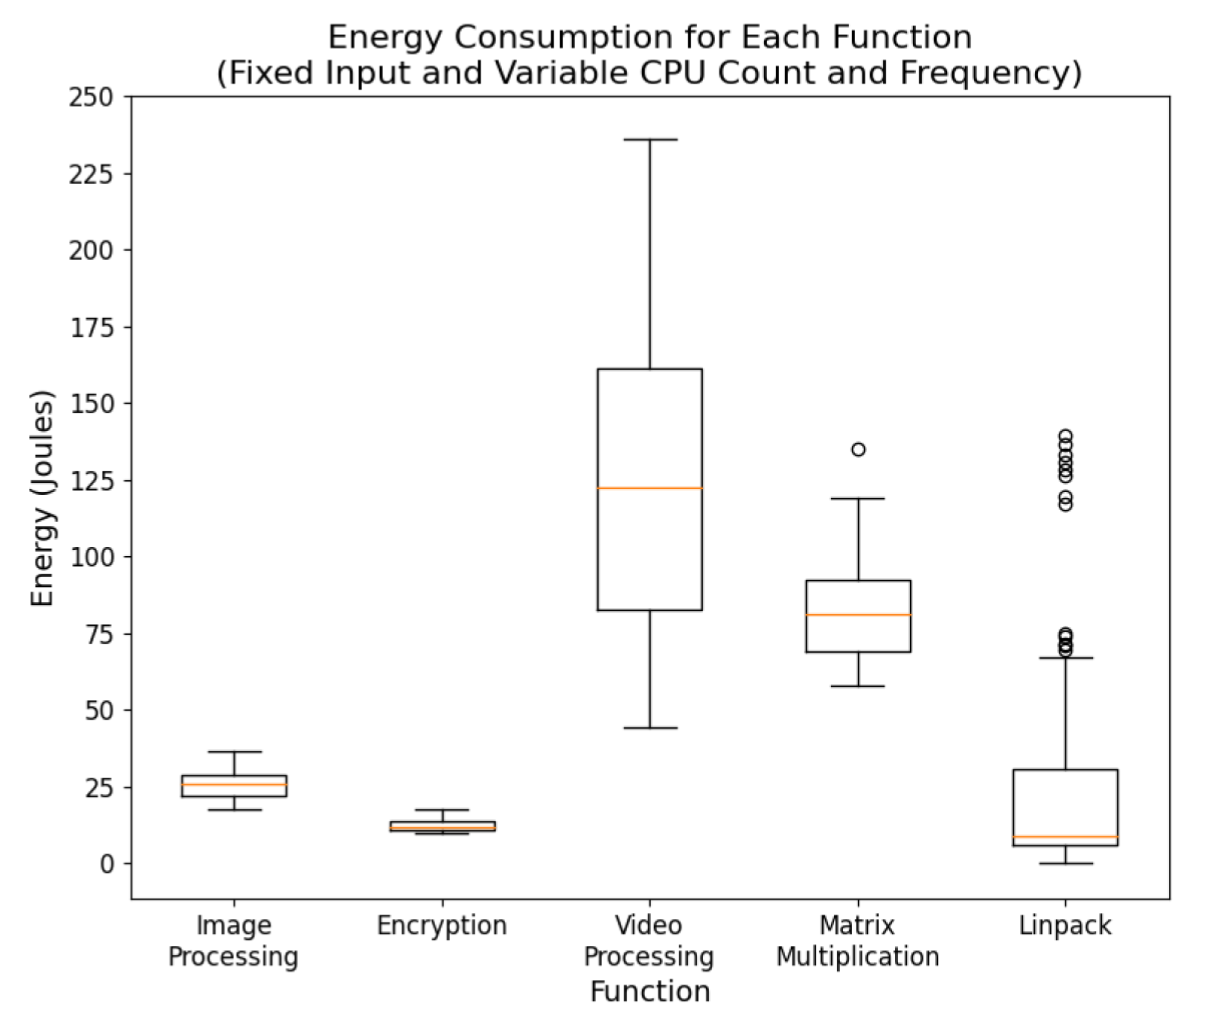
\includegraphics[width=0.45\textwidth]{imgs/energy_boxplot.png}
   \caption{Boxplot showing energy variability across functions with fixed input, while changing vCPU count and frequency. }
   \label{fig:energy_boxplot}
 \end{figure}
\section{Related Work}
% Include CherryPick and Aquatope
CherryPick \cite{CherryPick} is a framework that was developed to find optimal or near-optimal cloud configurations (vCPU and memory) for repetitive big data analytics jobs, addressing challenges of system cost, performance, and adaptivity. CherryPick leverages Bayesian Optimization (BO) to build performance models that are able to determine optimal or near-optimal configurations that satisfy performance constraints with a relatively low number of samples. 

Aquatope \cite{aquatope} also utilizes Bayesian models to optimize for resource allocation for serverless function invocations. This framework also utilizes BO to learn the mapping from resource configuration to performance and cost, while considering noise and uncertainty in the cloud environment. Aquatope also uses batch sampling to reduce the cost of exploration when finding a resource configuration.

Our work aims to draw from the ML techniques utilized in CherryPick and Aquatope. This is because the fundamental problem for us is very similar to both Aquatope and CherryPick, as we are optimizing for some value (in our case, energy) given a serverless function. We will also set performance constraints to ensure user-specified SLOs are met.

In the space of carbon-aware computing, GreenCourier \cite{GreenCourier} is a scheduling framework that enables runtime scheduling of serverless functions across geographically distributed regions based on their carbon efficiencies. This work focuses on minimizing carbon footprint based on the location at which a function is run, whereas our work aims to optimize the host environment through proper resource allocation and configuration to minimize carbon emissions using function-level characteristics.

\begin{table*}[htbp]
   \centering
   \begin{tabular}{|c|c|}
   \hline
   \textbf{Variable} & \textbf{Values} \\ \hline
   Function Type & Float Matrix Multiplication, Image Processing, Video Processing, Encryption, Linpack \\ \hline
   vCPU Count & 1, 2, 3, 5, 7, 10, 13, 16, 19, 22, 25, 28, 31 \\ \hline
   vCPU Frequency (GHz) & 1.0 to 2.4 in 0.2 increments\\ \hline
   \end{tabular}
   \caption{Measurement Study Configurations -- Energy Variation with vCPU and Frequency Allocation}
   \label{tab:mstudy1_configurations}
\end{table*}

\begin{table*}[htbp]
  \centering
  \begin{tabular}{|c|c|}
  \hline
  \textbf{Variable} & \textbf{Values} \\ \hline
  Image & main-python, video-ow, mobilenet-ow, sentiment-ow, audio-ow \\ \hline
  vCPU Count & 1, 2, 3, 4, 5, 6, 7, 8, 9, 10, 12, 14, 16, 18, 20, 22, 24, 26, 28, 30, 32 \\ \hline
  Memory (MB) & 512 to 10240 in 512 increments\\ \hline
  \end{tabular}
  \caption{Measurement Study Configurations -- Energy Variation with vCPU and Frequency Allocation}
  \label{tab:mstudy1_configurations}
\end{table*}

\section{Measuring Carbon Emission}


Before conducting the measurement study, we need to define how to measure carbon emissions. According to Gupta et al. \cite{gupta2022act}, the carbon footprint of a server can be calculated using the following formula where $OP_{CF}$ is the operational carbon footprint, $CI_{use}$ is the carbon intensity of the energy source, and $Energy$ is the operational energy:

\begin{equation}
   OP_{CF} = CI_{use} \times Energy
\end{equation}

The carbon intensity refers to how \textit{clean} the energy source is. For example, coal has a higher carbon intensity than solar. We assume that the energy source of the serverless system is constant, and therefore, the carbon intensity is constant. We can then use the operational energy as a proxy for the carbon footprint.

\subsection{Measuring Energy}
We first need a way to measure the energy consumption of a serverless function invocation. EnergAt \cite{he2023hotcarbon} is a tool that measures fine-grained energy consumption at the thread-level while taking into account Non-Uniform Memory Access (NUMA) effects. An EnergAt process continuously samples a target container, where each sample returns energy readings over an interval of at least 50ms. Therefore, EnergAt will get continuous back-to-back samples of energy readings over time. The energy consumption of a target container is the sum of the energy readings over the duration of the function invocation. One limitation of EnergAt is that every target container for which we want to measure energy consumption must be instrumented with its own EnergAt process. This is not feasible as the number of EnergAt processes and resource contention scales with the number of target containers.

To mitigate this issue, we created EnergyLiteDaemon. EnergyLiteDaemon is a daemon that samples multiple target containers in a round-robin fashion, where each sample returns energy readings over an interval of at least 50ms. This allows us to measure the energy consumption of multiple target containers with a single, lightweight, process. Due to the round-robin fashion, however, the sampling frequency per target container decreases as a function of the number of target containers. If there are multiple containers, the samples are no longer back-to-back -- there may be some time delay between two samples. To solve this, we complete the following steps to interpolate the total energy consumption of a target container:

\textbf{Power Calculation:} We compute the average power for every sample by dividing the energy consumed over the interval of the sample by the duration of that interval. This allows us to get a power-time scatter plot that contains $n$ points, where $n$ is the number of samples.

\textbf{Trapezoidal Integration:} Given a power-time scatter-plot, we compute the total energy consumption of a target container using trapezoidal integration. All of the points in the power-time scatter plot are connected by straight lines, and the area under the curve is calculated. This area is the total energy consumption of the target container. 

A toy example of energy measurement using EnergAt and EnergyLiteDaemon is shown in Appendix \ref{appendix:energy_measurement}.

Due to EnergyLiteDaemon's round-robin sampling approach, which reduces its overhead, it may not capture all energy readings for a container. Even with trapezoidal integration, the energy consumption will not be exact. To determine the accuracy of EnergyLiteDaemon, we ran 20 stress docker containers, with varying CPU usage and duration. Figure \ref{fig:EnergyLiteDaemon_Efficacy} shows the energy consumption of the containers as measured by EnergAt and EnergyLiteDaemon. The absolute percentage error of EnergyLiteDaemon is less than 15\%, which is acceptable for our purposes.

\begin{figure}[ht]
   \centering
   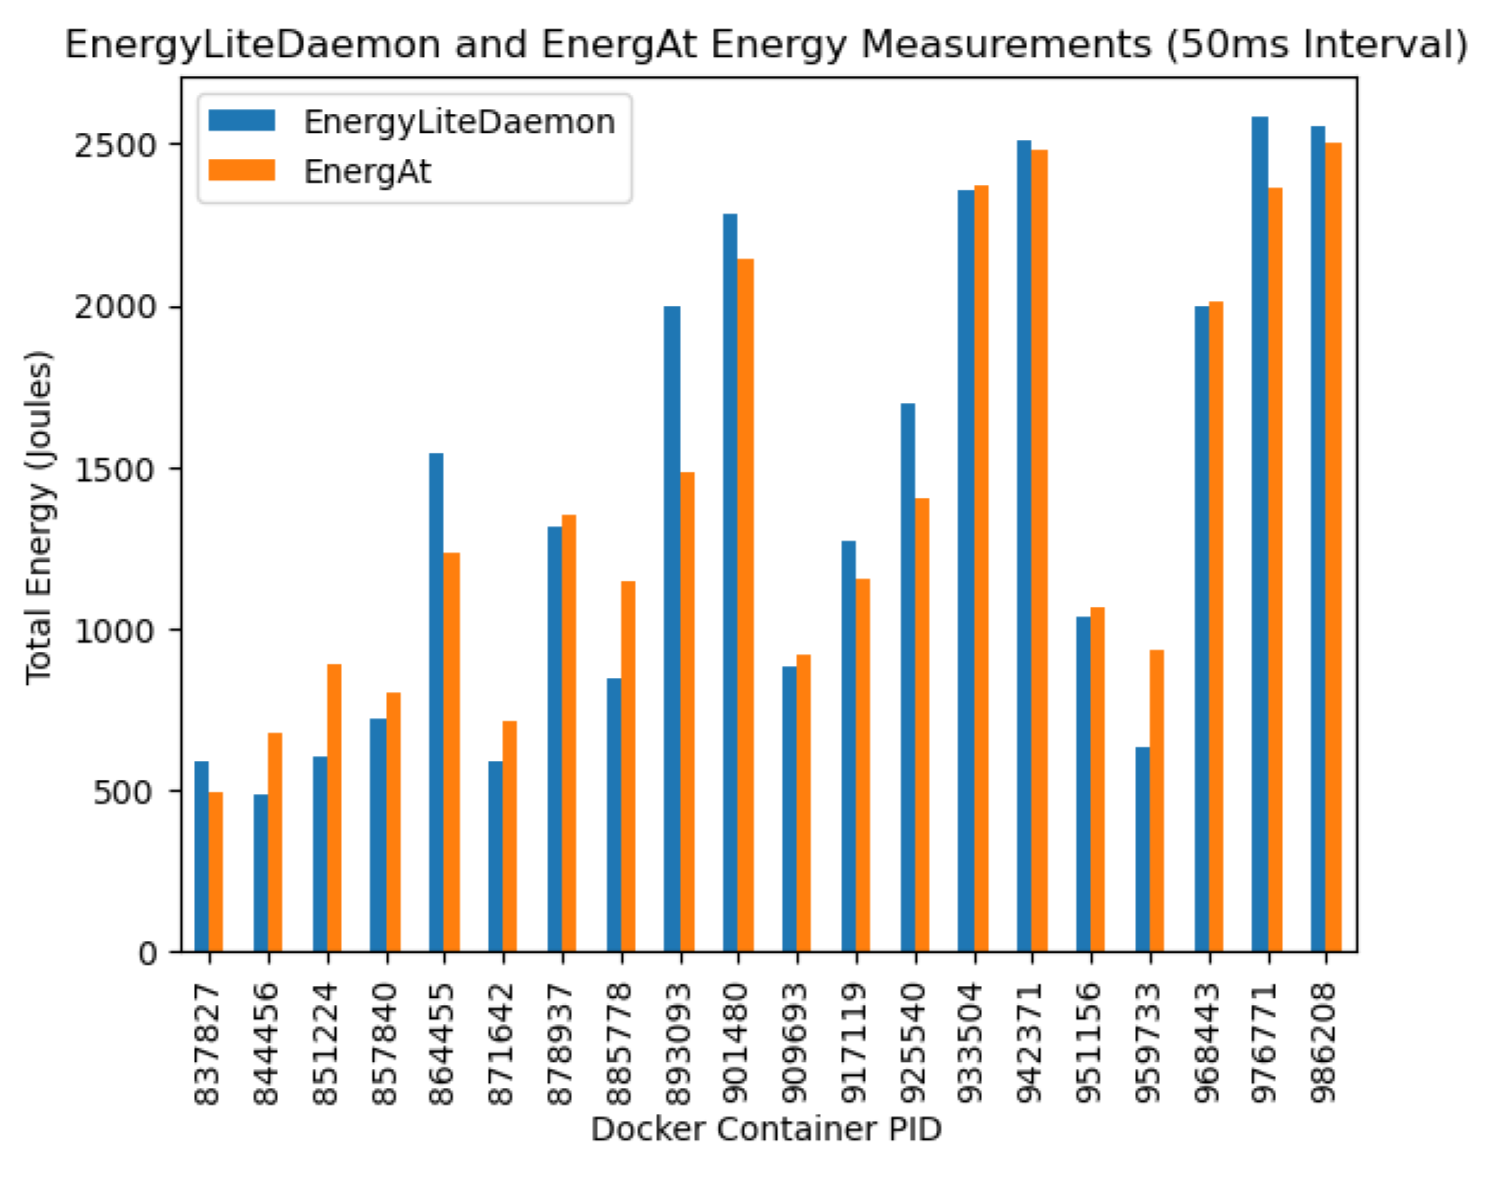
\includegraphics[width=0.45\textwidth]{imgs/EnergyLiteDaemon_Efficacy.png}
   \caption{Energy measurements of EnergAt and EnergyLiteDaemon for 20 stress docker containers.}
   \label{fig:EnergyLiteDaemon_Efficacy}
 \end{figure}

\section{Measurement Study}

We conduct two measurement studies to answer the following questions: \textbf{1. How does energy vary with changes in vCPU and frequency allocation? 2. What is the energy consumption over the lifecycle of a serverless function invocation?}

To perform the measurement study, we use OpenWhisk, which is an open-source serverless platform, to run function invocations. We use EnergyLiteDaemon to measure the energy consumption of the function invocations.

\subsection{Energy Variation with vCPU and Frequency Allocation}

A variety of workloads were run on different vCPU and frequency configurations. We collected the vCPU utilization, energy consumption, and performance in terms of duration. The resource configurations are shown in Table \ref{tab:mstudy1_configurations}.

We then analyzed the data to understand how energy consumption varies with changes in vCPU and frequency allocation. For float matrix multiplication, energy usage initially decreases and then tends to plateau as the vCPU allocation increases. This is because matrix multiplication is highly parallelizable and has high vCPU utilization, leading to a decrease in duration and energy usage. For image processing, energy usage has no apparent correlation with vCPU allocation, likely because most of the image processing tasks are non-parallelizable. For encryption, energy usage, duration, and vCPU utilization do not change with vCPU allocation because encryption is also non-parallelizable and does not benefit from additional vCPUs.

For both types of functions, energy consumption as a function of frequency displays a convex relationship, where energy consumption decreases with frequency until a certain point (which varies between different functions and function inputs), and then begins to increase again. This is because the energy consumption per time unit of a vCPU is proportional to the frequency at which it runs, but the overall duration of the function is inversely proportional to the frequency at which the vCPU runs. 

For functions that are non-parallelizable, we wanted to assess whether the optimal frequency to run an invocation is the same across all function inputs (since vCPU count is not as big of a factor as in parallelizable functions). However, across various inputs, we found that the frequency that results in minimum energy expended varies. 

All of these findings support the idea that we should use machine learning to learn the relationship between vCPU, frequency, and energy consumption, and use this model to minimize energy consumption while meeting SLOs.

More details on the results can be found in Appendix \ref{appendix:energy_variation_vcpu_frequency}.

\subsection{Energy Consumption Over the Lifecycle of a Serverless Function Invocation}
Additionally, we ran a variety of docker images, each of a different size, with a variety of vCPU and memory configurations to investigate carbon emissions of different stages of the container lifecycle. For each (image, vCPU, memory) configuration, we measured the energy consumption at different stages of the function invocation lifecycle. More specifically, we measured the energy consumed during the container spin-up, the idle time, and the container spin-down.

After collecting and analyzing the data, we first found that for each stage of the lifecycle we measured, when changing the vCPU and memory configurations, the energy consumption did not vary significantly. This was true for all image sizes. This is likely due to the fact that these resources will not actually be allocated to the container until the compute inside the container requires them. We did notice that if we varied the image size, the energy consumption of the container spin-up process significantly increased as the image size increased. However, it is worth noting that most of the energy consumption of the spin-up is accredited to the `docker pull' process, which would only be a one-time operation. The `docker run' does not consume a significant amount of energy and does not show any statistical correlation. For the idle time, we noticed a strange negative correlation trend with the image size, and for the spin-down, we noticed a somewhat positive correlation with a few outlier points. Since we only used a few image sizes, we cannot definitively conclude that these trends will extrapolate.

Due to our findings of little to no correlations, we decided to not pursue a carbon-aware keep-alive policy further. More details on the study can be found in Appendix \ref{appendix:energy_variation_vcpu_memory}.

\section{Final System}

Our final system, Carbon Aware Serverless System (CASS), consists of two main components: a machine learning model that predicts the optimal vCPU count and frequency for a given function invocation, and a custom scheduler that attempts to route the invocation to a warm container with or greater than the predicted vCPU count and frequency.

\subsection{Machine Learning Model}
To implement a machine learning model to minimize carbon emissions, we utilize a Gaussian Process Regressor (GPR), similar to Aquatope\cite{aquatope}. GPR uses the same mathematical foundation as Bayesian Optimization (BO), resulting in it having the same advantages as BO, including not needing a lot of data points to train and having online learning capabilities. In addition, by using the regression model, we can use the vectorized function input as an additional feature for the model and test different resource configurations while fixing the function input to find the minimum energy for a specific invocation. In our final implementation, we utilize the Matern kernel, which offers more flexibility in modeling smoothness and can help better capture relationships between different inputs when the function is not smooth everywhere, and the white kernel, to model noise. 

Using our model, we optimize for vCPU allocation and operational frequency to try and minimize carbon emissions, while setting SLOs as our constraint. Since we have collected data on 5 different functions and each function has different usage patterns, we have a separate model for each function. Each function's input is encoded into an input vector for the regression model, and the vCPU count and frequency are concatenated to this input vector.

When a function is invoked, after the input feature vector is constructed, we perform an iterative process in which we go through all possible resource configurations (in terms of vCPU count and frequency) and predict the energy consumption and duration for that specific function and function input given the configuration. Given these predictions, we filter the results that were predicted to violate SLOs, and choose the vCPU count and frequency configuration that minimizes the energy consumption. 

Since our model is trained from scratch, early inferences by the model will have lower confidence. To encourage exploration of the feature space in early invocations of a function and allow the model to see a more diverse set of data points for training, we set the value for a confidence threshold that the model prediction should meet. In the case that the prediction is not confident, we sample a random configuration of resources for the invocation to run at. 

Simultaneously, we have a background thread that is periodically polling a database that receives observed energy and latency readings from our invokers and uses this as training data to train our models, to utilize online learning. This, however, is not on the critical path.



A diagram of the machine learning model is shown in Figure \ref{fig:ml_model}.

\begin{figure}[ht]
   \centering
   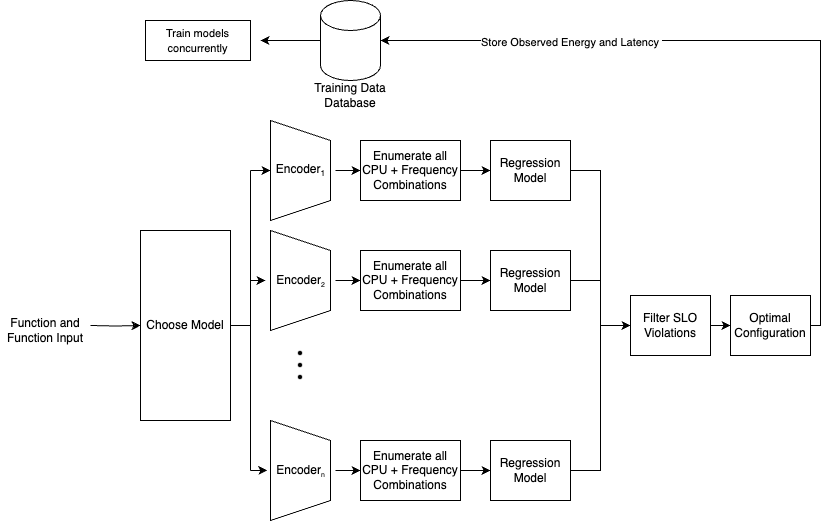
\includegraphics[width=0.45\textwidth]{imgs/ml_model.png}
   \caption{Gaussian Process Regression Model for Carbon-Aware Serverless System}
   \label{fig:ml_model}
 \end{figure}

 \subsubsection{Evaluating Model Performance on Measurement Study Data}
In order to analyze the effectiveness of our model and tune hyperparameters, such as the confidence threshold and the type of kernel used, we simulate a trace of function invocations using the measurement study data and compare our model predictions to the ground truth values obtained from the study.

Every ten seconds, we ``invoke" a function with a certain function input and send this information to the model, which vectorizes the function input features and finds the optimal resource configuration that meets SLOs. Our model is trained simultaneously in a background thread every 30 seconds. 
 
For Float Matrix Multiplication, Linpack, and Encrypt, our model is able to eventually converge to a minimum energy value after training on a certain number of invocations and learning from the patterns that it sees overtime. We analyze the energy expended over time for each function invocation (for a few function inputs) and see a clear convergence for these three functions. When comparing the energy consumption of the predicted configuration to the energy of the known minimum configuration (from our ground truth values), we also see the difference between these two values eventually converge to a value close to 0. (meaning our prediction of the optimal configuration is very close to the actual minimum configuration). 

We also assess the model predictions themselves by calculating the difference in the energy that is predicted for a certain configuration vs the actual energy expended for that configuration. For these three functions, we see the model can eventually predict accurate energy values for a function given the function input and configuration of resources.

However, for image processing and video processing, our results are far more unstable and don't show clear signs of convergence in any of these aspects (energy over time, energy of predicted configuration vs minimum configuration, energy predicted by model vs ground truth energy). As we saw in the measurement study, the correlation between energy, function input, and vCPU count and frequency was more unpredictable/unclear compared to the previously discussed functions. Therefore, the model proved to have a more difficult time finding optimal resource configurations and had lower confidence in its predictions, leading to a higher amount of random configurations being chosen. 

The figures that contain details on this analysis can be found in Appendix \ref{appendix:regression_model_measurement_study}.


\subsection{Adapting OpenWhisk}

\begin{figure}[ht]
   \centering
   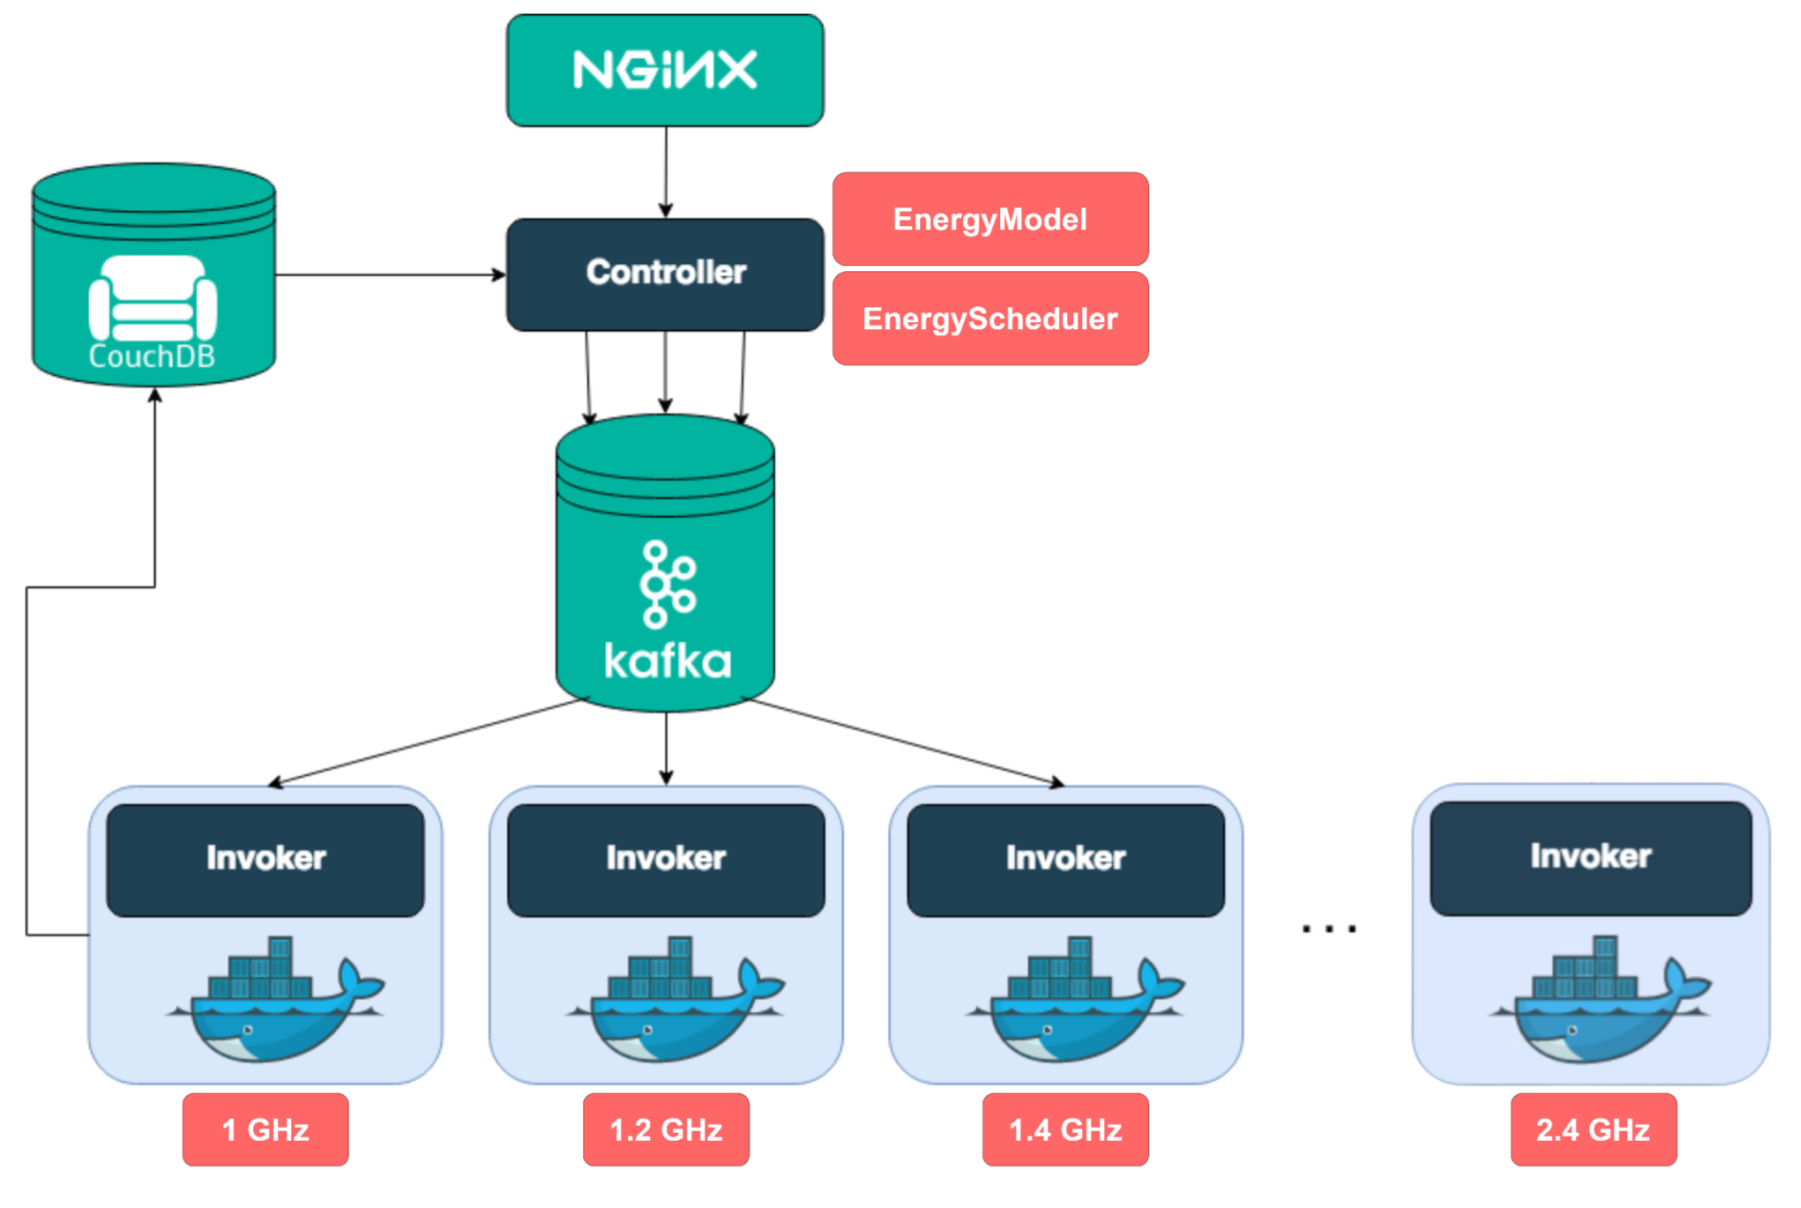
\includegraphics[width=0.45\textwidth]{imgs/Adapted_OW_System_Overview.png}
   \caption{Adapted OpenWhisk System Overview}
   \label{fig:adapted_ow_system_overview}
 \end{figure}

We adapted OpenWhisk to incorporate Gaussian Process Regression to drive a carbon-aware DFS and vCPU allocation model. Figure \ref{fig:adapted_ow_system_overview} shows the system overview.

The Gaussian Process Regression model is contained in a shim layer, called the EnergyModel. Whenever a user invokes a function, the EnergyModel determines the optimal vCPU and frequency allocation. The EnergyModel is trained online periodically at 30 second intervals.

We created a custom scheduler, called EnergyScheduler, that replaces OpenWhisk's current scheduler. There are multiple invoker nodes, each running at a different frequency, as shown in Figure \ref{fig:adapted_ow_system_overview}. The EnergyScheduler uses the output of EnergyModel to determine which invoker to send the function invocation to. We base the EnergyScheduler's algorithm off of Shabri's scheduler \cite{sinha2024shabari}. EnergyScheduler is designed to mitigate cold starts by:

\textbf{1. Prioritizing routing the invocation to warm containers: } The scheduler will receive the invocation and the predicted vCPU and frequency allocation from the EnergyModel. The scheduler will then iterate through the invokers running at at least the predicted frequency and attempt to find a warm container that is closest to the predicted vCPU allocation. If a warm container is found, the invocation is sent to that container. If no warm container is found, the invocation is sent to the invoker running at the predicted frequency.

\textbf{2. Preemptively spinning up containers: } In the case that the invocation is sent to an invoker running at higher than the predicted frequency or with more vCPUs than predicted, the scheduler will preemptively spin up a container on the invoker running at the predicted frequency with the predicted vCPU allocation. This is done to mitigate future cold starts and underutilization of resources. The underlying assumption is that function invocations exhibit temporal locality, meaning that in a short time frame, the same function is likely to be invoked again. Thus, preemptively spinning up a container will reduce the likelihood of cold starts for future invocations and underutilization of resources.

\section{Evaluation}

\subsection{Methodology}
\textbf{Workloads.} We evaluate our system using functions shown in Table \ref{tab:summary_of_serverless_functions}. These are the same functions used in the measurement study. These functions vary in their parallelizability and resource requirements, making them suitable for evaluating the effectiveness of our system. We utilize the same Azure trace used in Shabri \cite{sinha2024shabari} to simulate function invocations, which is a scaled down sample of the Azure trace. We utilize a requests per second (RPS) of 1 for the evaluation.

\begin{table*}[htbp]
  \centering
  \begin{tabular}{|c|c|c|c|c|}
  \hline
  \textbf{Function} & \textbf{Input Type} & \textbf{\# Runs} & \textbf{Sizes} & \textbf{Size Range} \\ \hline
  floatmatmult & square matrix & 383 & 25 & 1000 - 8000 \\ \hline
  linpack & square matrix & 381 & 22 & 250 - 10000 \\ \hline
  encrypt & string & 348 & 36 & 500 - 50000 \\ \hline
  imageprocess & image & 374 & 64 & 916K - 30M \\ \hline
  videoprocess & video & 358 & 17 & 284K - 11M \\ \hline
  \end{tabular}
  \caption{Summary of serverless functions used in experiment}
  \label{tab:summary_of_serverless_functions}
\end{table*}

\textbf{Metrics.} For a high-level, comprehensive evaluation of our system compared to baseline models, we aggregate all of the energy readings for each function invocation for a specific function type (as the overall energy expended for that function) and compare these energy totals across each model. We also count the total number of SLO violations for each function type and compare this across all models as well.

\textbf{Baselines.} We compare our system to two baselines Parrotfish and Aquatope. Parrotfish \cite{parrotfish} utilizes parametric regression to predict resource configuration, while Aquatope \cite{aquatope} uses Bayesian Optimization to predict resource configuration. Neither of the aforementioned baselines consider optimizing for energy efficiency. Furthermore, the original OpenWhisk's scheduler was used when running Parrotfish and Aquatope. Parrotfish only optimizes memory allocation; thus, we allocate CPU proportional to memory. 

\textbf{Our System.} Since our system, CASS, only optimizes CPU and frequency, we run our system with two memory configurations: 1. using Parrotfish's memory predictions (CASS\_Parrotfish), 2. using Aquatope's memory predictions (CASS\_Aquatope). We compare our system to the aforementioned baselines in terms of energy consumption and SLO violations.

\subsection{Assessing the Efficacy of EnergyLiteDaemon for Collecting Energy Readings}

Before running the full evaluation of our regression model and scheduler, we ran a preliminary evaluation of our energy measurement tool, EnergyLiteDaemon, on the Azure trace, in terms of how effectively and accurately it can collect energy readings for each function invocation. We compared its results to the original implementation of EnergAt.  

As shown in Figure \ref{fig:energy_tool_efficacy}, EnergyLiteDaemon has far more invalid energy readings compared to EnergAt. Invalid is defined as a negative reading, which signifies that no energy measurements were collected during the lifecycle of that function invocation, or the energy measured was 0. The reason EnergyLiteDaemon has far more invalid readings is that unlike EnergAt, which has a dedicated process energy measurement process per active container, EnergyLiteDaemon only consists of a single process that loops through all the active containers and iteratively samples for energy for each container for a specified period of time. When there are hundreds of containers that are running simultaneously, there is a high likelihood that the EnergyLiteDaemon is not able to collect energy samples for functions with shorter durations before they complete. 

\begin{figure}[H] % Note the use of figure* instead of figure
   \centering
   \begin{subfigure}[b]{0.5\textwidth} % Adjusted width to fit across two columns
         \centering
         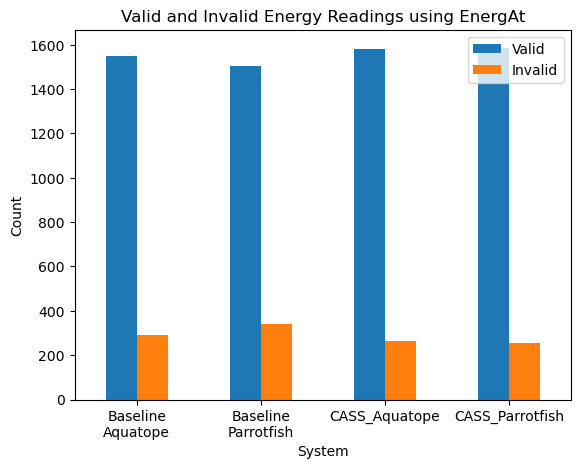
\includegraphics[width=0.6\linewidth]{imgs/final_experiment_plots/valid_vs_invalid/EnergAt.png}
         \caption{EnergAt}
         \label{fig:energy_tool_efficacy_a}
   \end{subfigure}
   \begin{subfigure}[b]{0.5\textwidth} % Adjusted width
         \centering
         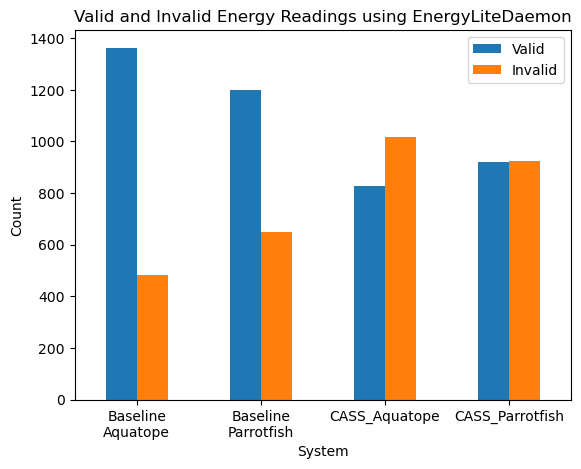
\includegraphics[width=0.6\linewidth]{imgs/final_experiment_plots/valid_vs_invalid/EnergyLiteDaemon.png}
         \caption{EnergyLiteDaemon}
         \label{fig:energy_tool_efficacy_b}
   \end{subfigure}
   
   \caption{Comparing the number of invalid vs valid energy readings for EnergyDaemonLite and EnergAt}
   \label{fig:energy_tool_efficacy}
\end{figure}

Though EnergAt is more computationally expensive and could lead to resource contention, for collecting accurate energy values, it was the most practical tool to incorporate into our system. To alleviate the issues associated with EnergyLiteDaemon, possible future steps that could be taken to improve the tool include reducing the energy sampling period, refining the interpolation technique used, and settling on a middle ground of having a separate process for each set of 20 or so containers, rather than having only 1 process for all containers or having 1 process per container. Furthermore, the current implementation of EnergyLiteDaemon is in Python; rewriting it in a lower-level language such as C++ could also help speed up the process of collecting energy readings.

\subsection{Results using EnergAt}

Due to EnergyLiteDaemon's inability to collect accurate energy readings with many containers, for the rest of the evaluation, we used EnergAt as our energy measurement tool and evaluated the efficacy of our end-to-end system in terms of conserving energy while meeting SLOs. 

\subsubsection{Energy Comparison}
For a given specific function type, we add up the energy readings for each invocation and use that as the metric for the total amount of energy consumed for that function type. Figures \ref{fig:cassvsaquatope_energy} and \ref{fig:cassvsparrotfish_energy} show the comparison between the Carbon Aware Serveless System (CASS\_Aquatope) and Aquatope, as well as CASS\_Parrotfish and Parrotfish, respectively. 


\begin{figure}[H] % Note the use of figure* instead of figure
   \centering
   \begin{subfigure}[b]{0.5\textwidth} % Adjusted width to fit across two columns
         \centering
         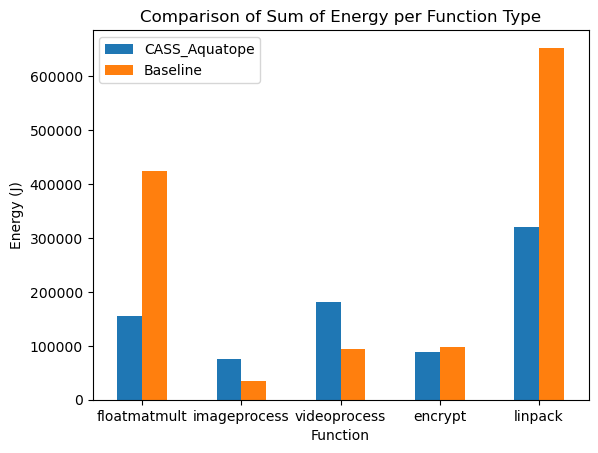
\includegraphics[width=0.6\linewidth]{imgs/final_experiment_plots/energy_comparison/aquatope/overall.png}
         \caption{Overall energy expended for CASS\_Aquatope vs Aquatope}
         \label{fig:cassvsaquatope_energy}
   \end{subfigure}
   \begin{subfigure}[b]{0.5\textwidth} % Adjusted width
         \centering
         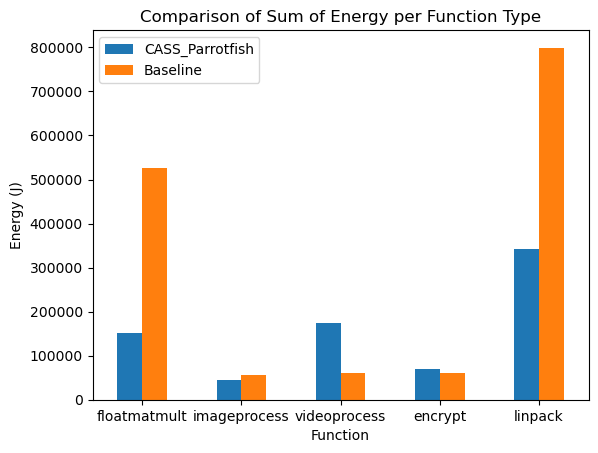
\includegraphics[width=0.6\linewidth]{imgs/final_experiment_plots/energy_comparison/parrotfish/overall.png}
         \caption{Overall energy expended for CASS\_Parrotfish vs Parrotfish}
         \label{fig:cassvsparrotfish_energy}
   \end{subfigure}
   \caption{}
\end{figure}

As shown in the figures, the functions that are highly parallelizable and have a clear underlying correlation between the relevant input features (such as vCPU count) and energy consumption, such as Float Matrix Multiplication and Linpack, see a reduction in energy consumption by almost 50\% compared to both baseline models. Encrypt sees comparable energy between the CASS and the two baselines, whereas Image Processing and Video Processing see worse energy consumptions compared to both baselines.

For Encrypt, as shown in our analysis of our model on the measurement study data, the model was able to converge to an optimal resource configuration (in terms of energy consumption) after several hundred invocations per function given a specific input. Because the Azure trace only contained a few hundred invocations per function type, and only a handful for a specific function input, we were not able to see the model learn to its full capacity. Given more function invocations to train on, we believe we could see a reduction in energy consumption comparable to Float Matrix Multiplication and Linpack.

For Image Processing and Video Processing, we can likely attribute this decrease in performance in terms of energy consumption to the highly complex relationships between energy consumption and the function input and resources allocated. As discussed in the measurement study section, there are no clear trends or correlations that could be seen, and for the model to predict configurations with high confidence (if at all possible), it would require far more function invocations for it to learn from. 

After doing further analysis, we concluded that the model provides the scheduler random configurations due to the low confidence in its energy predictions, which is most likely what leads to large fluctuations in energy consumption. In our current implementation, if the configuration with the minimum energy has low confidence, we immediately choose a random configuration. For future improvements, we can instead check the top k configurations (where k is a hyperparameter) and choose the best configuration that meets the confidence threshold (and choose a random configuration if none of them meet the threshold). This optimization may help improve the energy expenditure of the overall system. 

Figures containing the energy difference between CASS and the baselines for each function invocation in the trace can be found in \ref{appendix:end-to-end_analysis}

\subsubsection{SLO Violations Comparison}

For each function type, we also calculate the number of invocations that violate the specified SLO. Figures \ref{fig:cassvsaquatope_slo} and \ref{fig:cassvsparrotfish_slo} show the comparison between CASS\_Aquatope and Aquatope, as well as CASS\_Parrotfish and Parrotfish, respectively. 


\begin{figure}[H] % Note the use of figure* instead of figure
   \centering
   \begin{subfigure}[b]{0.5\textwidth} % Adjusted width to fit across two columns
         \centering
         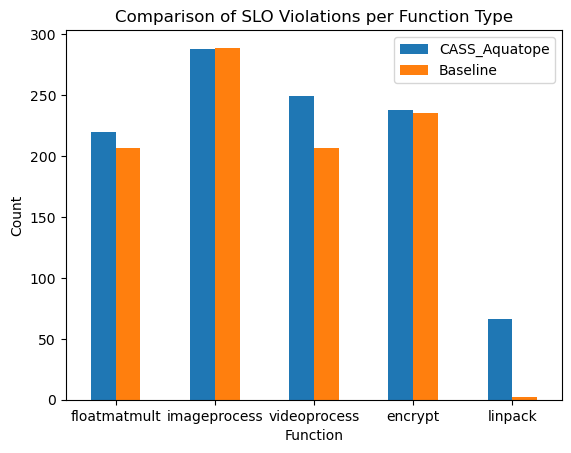
\includegraphics[width=0.6\linewidth]{imgs/final_experiment_plots/duration_comparison/aquatope.png}
         \caption{Number of SLO violations for CASS\_Aquatope vs Aquatope}
         \label{fig:cassvsaquatope_slo}
   \end{subfigure}
   \begin{subfigure}[b]{0.5\textwidth} % Adjusted width
         \centering
         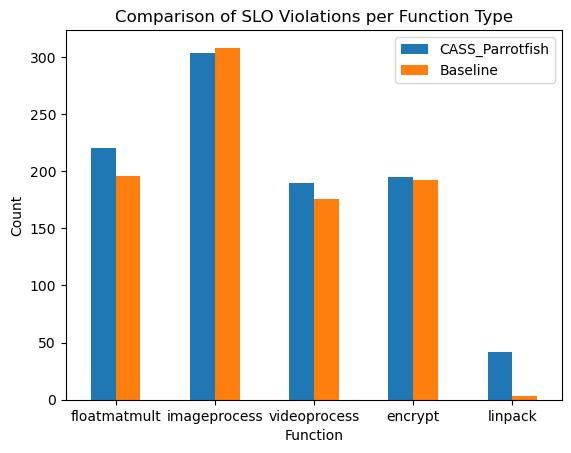
\includegraphics[width=0.6\linewidth]{imgs/final_experiment_plots/duration_comparison/parrotfish.png}
         \caption{Number of SLO violations for CASS\_Parrotfish vs Parrotfish}
         \label{fig:cassvsparrotfish_slo}
   \end{subfigure}
   \caption{}
\end{figure}

Overall, CASS has slightly more SLO violations than the baseline models for the different function types. However, overall, the number is comparable across CASS and the baseline models, except for Linpack. 

We can likely attribute the increase in SLO violations to the random configurations provided to the scheduler in the case of low confidence or generally poor predictions in early stages of training. For future works, we could try to incorporate a mechanism that can optimize the performance in a different aspect, such as increased CPU and memory utilization or lower latencies (similar to the baselines), if the EnergyModel is not able to confidently make predictions to minimize energy. This could help reduce the total number of SLO violations. 



\subsubsection{Model Overhead}

Since the model has to make predictions for every possible resource configuration before outputting the optimal configuration to the scheduler, the critical path incurs some overhead during the prediction process. The average overhead per function type can be seen in \ref{fig:cass_aquatope_overhead} and \ref{fig:cass_parrotfish_overhead}. The overhead is trivial compared to the actual durations of the functions invoked for this study and likely does not have a significant impact on the number of SLO violations. However, this overhead can still be reduced in future works by incorporating multithreading in the inference process. 

\begin{figure}[H] % Note the use of figure* instead of figure
   \centering
   \begin{subfigure}[b]{0.5\textwidth} % Adjusted width to fit across two columns
         \centering
         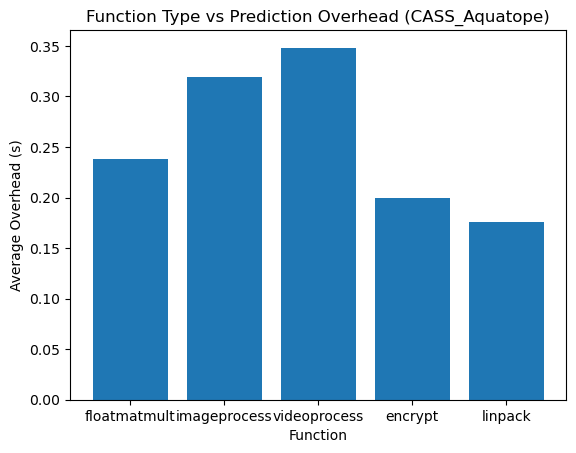
\includegraphics[width=0.6\linewidth]{imgs/final_experiment_plots/model_analysis/prediction_overhead/cass_aquatope.png}
         \caption{Prediction overhead for CASS\_Aquatope}
         \label{fig:cass_aquatope_overhead}
   \end{subfigure}
   \begin{subfigure}[b]{0.5\textwidth} % Adjusted width
         \centering
         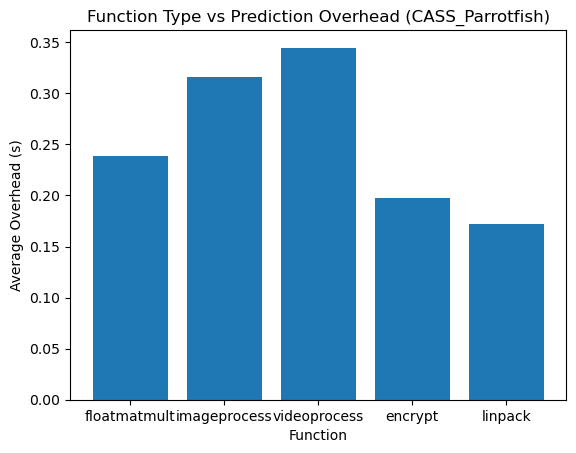
\includegraphics[width=0.6\linewidth]{imgs/final_experiment_plots/model_analysis/prediction_overhead/cass_parrotfish.png}
         \caption{Prediction overhead for CASS\_Parrotfish}
         \label{fig:cass_parrotfish_overhead}
   \end{subfigure}
   \caption{}
\end{figure}


\section{Discussion}
\textbf{EnergyLiteDaemon:} As discussed previously, EnergyLiteDaemon was not effective in collecting energy measurements for a large number of containers running simultaneously, which prompted us to switch back to EnergAt. Though EnergAt provides more accurate, realistic results, it introduces high overhead and resource contention, which may not be scalable as the RPS increases significantly in real systems. Future works would involve an improved energy collection method, which includes using C++ instead of Python and using an EnergyLiteDaemon process for a fixed number of containers, and adding new EnergyLiteDaemon processes for more containers. 

\textbf{Model Improvement:} Our model currently works well for improving energy consumption of functions such as Float Matrix Multiplication and Linpack, which have more straightforward correlations between resource configurations and energy usage. Future works would entail improving the model to be able to capture more complex relationships, which would improve the predictions for Image Process, Video Process, and Encrypt. Some ways to improve the model would be to refine the way the model handles predictions with low confidence; rather than defaulting to a random configuration if the best configuration has low confidence, we can assess the next best configuration as well. We can also perform a deeper analysis of the input features that have the biggest impact on the predictions made by the model and introduce some type of feature extraction or feature engineering to construct more informative inputs. 

\textbf{Practicality of End-to-End System} In our system currently, each invoker runs at a specific frequency, and invocations are sent to the invoker running at the frequency predicted by the model. This approach is not as practical if the number of invocations is scaled up significantly and invocations get routed to the same invokers repeatedly and cause increased traffic, which could occur due to temporal locality, which is when similar invocations are likely to occur multiple times. Instead, we can dynamically scale frequency by pinning containers to cores running at certain frequencies, where multiple cores may run at multiple frequencies on a single machine. This can also help prevent under-utilization of resources and improve SLO attainment.

Additionally, currently, the EnergyModel sequentially makes inferences for all CPU and frequency configurations, which introduces an overhead of up to 35ms on average. To alleviate this overhead, we can multithreaded the inference process on the controller side, which is an optimization that can reduce the overall latency of the critical path of the function invocation. 

\section{Conclusion}

In this paper, we introduce CASS, a Carbon Aware Serverless system that aims to minimize the carbon footprint of function invocations while continuing to meet service-level objectives. Throughout this work, we explore tools to collect energy measurements on a process-level, run a measurement study on different functions with various resource configurations to understand underlying patterns, and build an end-to-end system consisting of a Gaussian Process Regressor to predict the optimal resource configuration that minimizes energy and an Energy-Aware scheduler that routes the invocation to the correct invoker. Our evaluation shows that for functions with clear correlation between function inputs, resources, and energy expended, we can reduce the energy consumption by almost 50\% compared to existing baselines, while having comparable performance in terms of meeting SLO requirements. 


% \section{Conclusion}

\bibliographystyle{latex8}
\bibliography{latex8}

\appendix
\section{Appendix}
\subsection{Energy Measurement}
\label{appendix:energy_measurement}
A toy example of the energy measurement of a container using EnergAt and EnergyLiteDaemon is shown in Figure \ref{fig:energy_toy_example}. Figure \ref{fig:a} shows the energy readings of EnergAt. Figure \ref{fig:b} shows the energy readings of EnergyLiteDaemon. EnergyLiteDaemon doesn't capture all energy readings for the container due to the round-robin sampling approach. Figure \ref{fig:c} shows EnergyLiteDaemon's power calculation of each energy sample. Figure \ref{fig:d} shows the energy interpolation of EnergyLiteDaemon using trapezoidal integration.

\begin{figure*}[ht] % Note the use of figure* instead of figure
   \centering
   \begin{subfigure}[b]{0.24\textwidth} % Adjusted width to fit across two columns
         \centering
         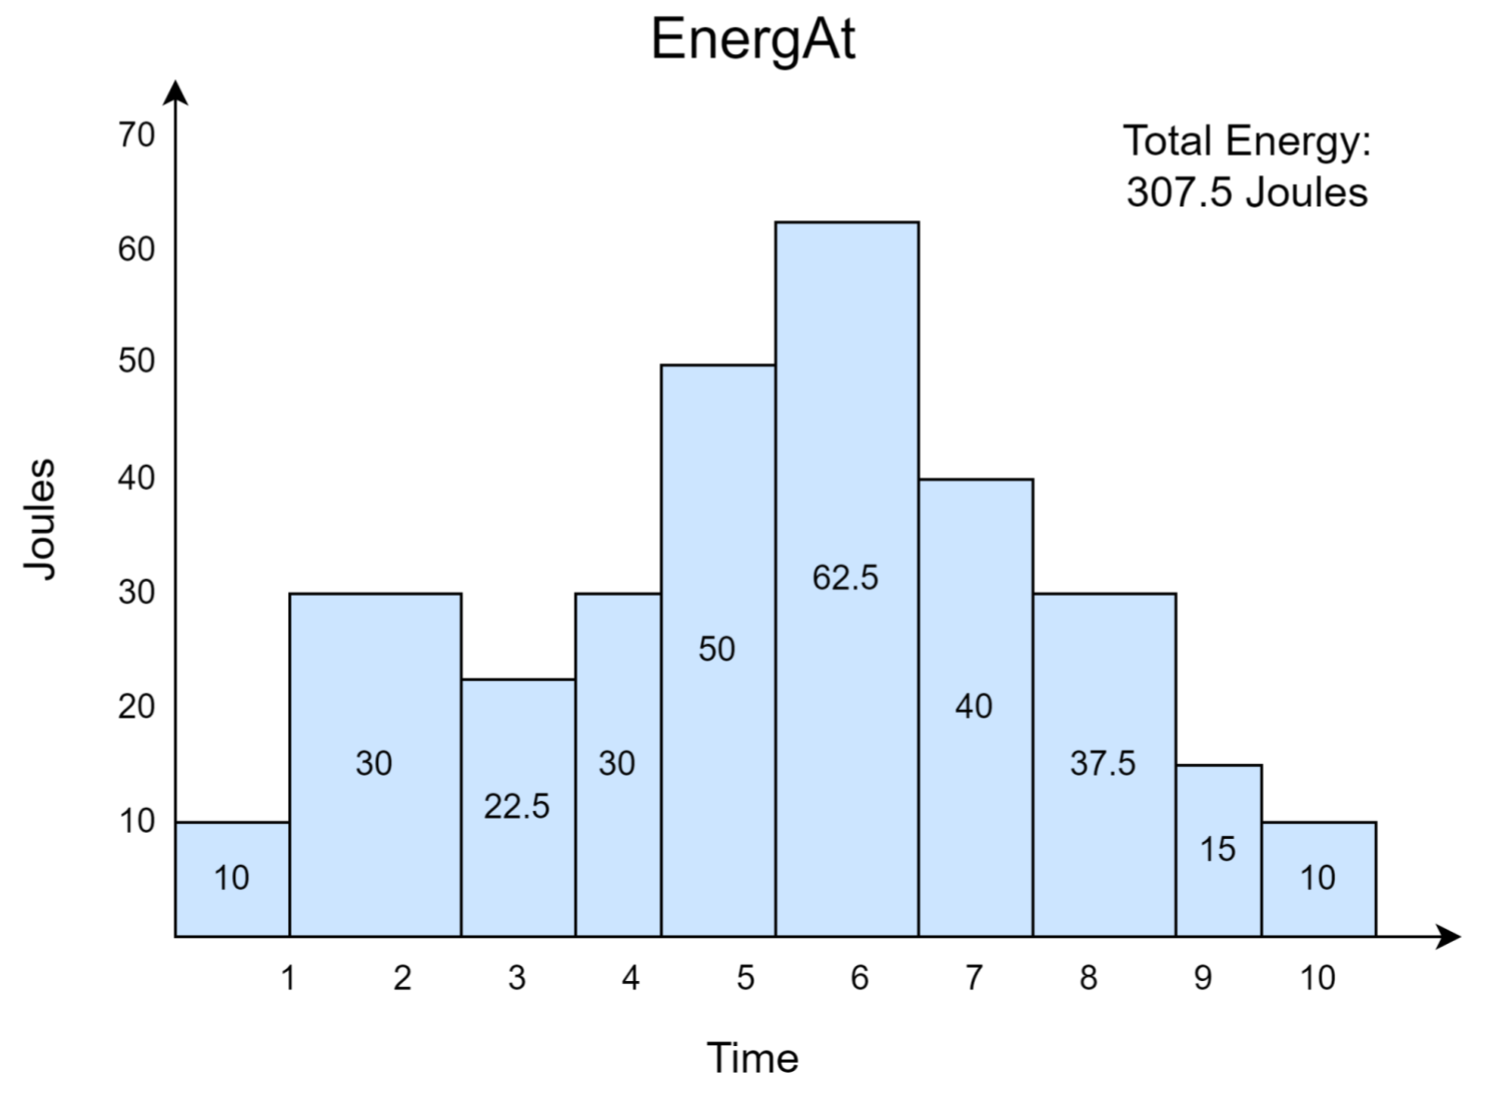
\includegraphics[width=\textwidth]{imgs/EnergAt_Energy.png}
         \caption{}
         \label{fig:a}
   \end{subfigure}
   \hfill
   \begin{subfigure}[b]{0.24\textwidth} % Adjusted width
         \centering
         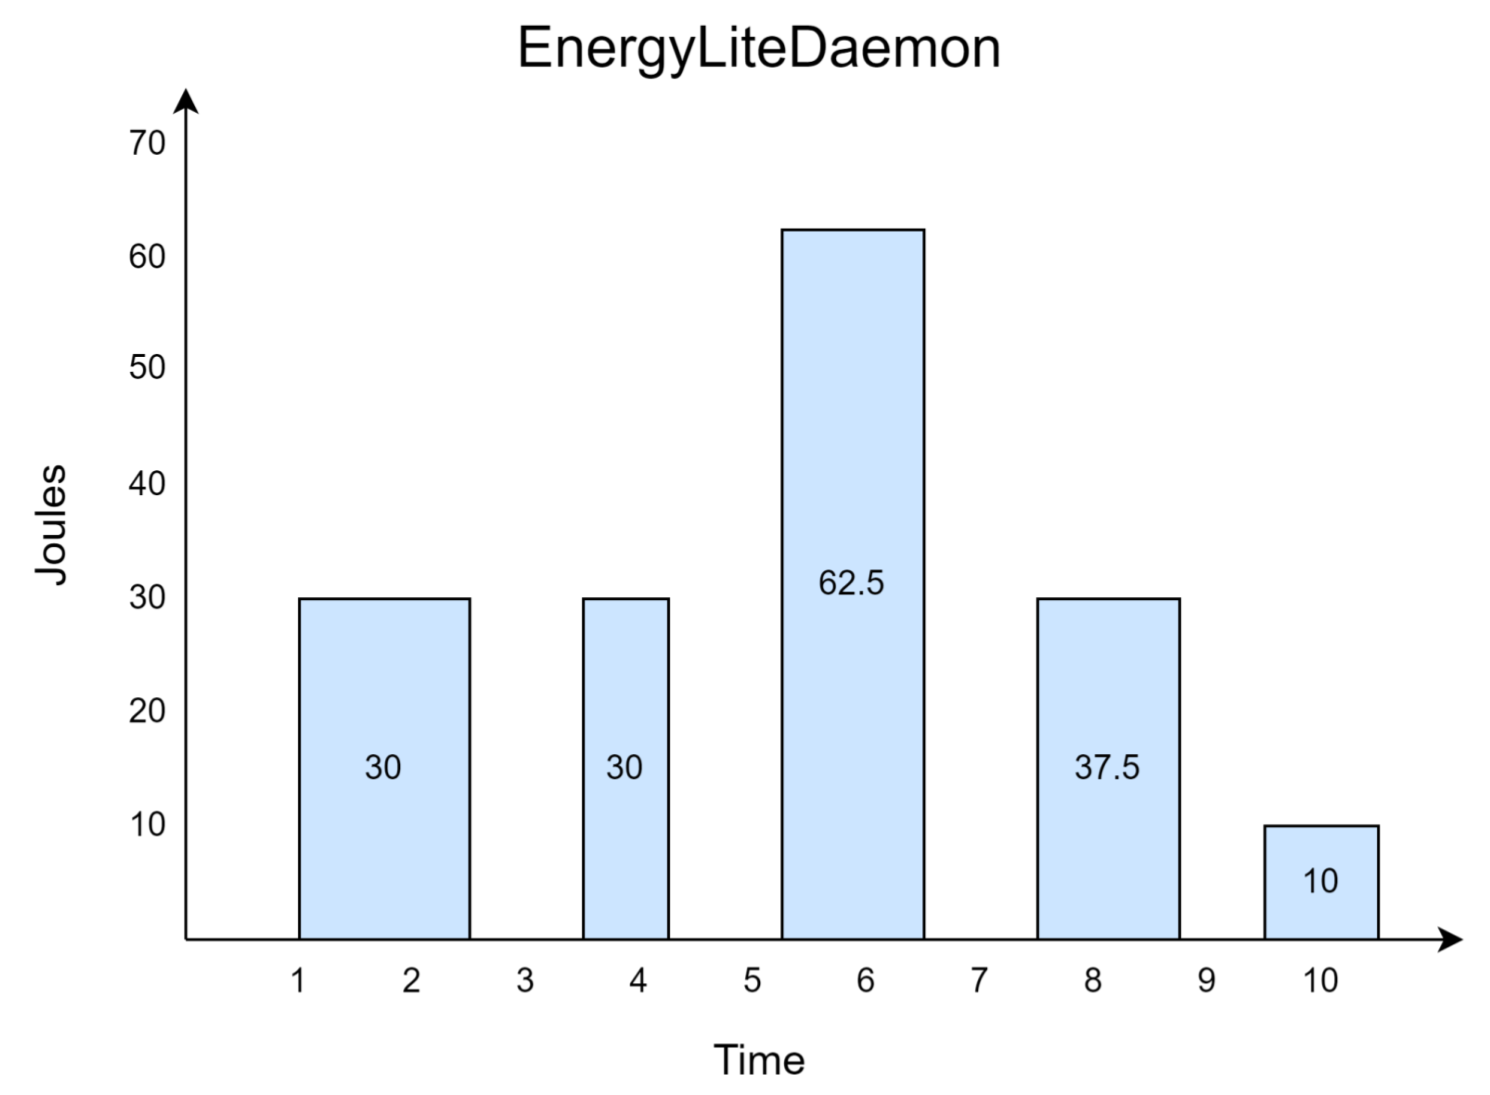
\includegraphics[width=\textwidth]{imgs/EnergyLiteDaemon_Energy_1.png}
         \caption{}
         \label{fig:b}
   \end{subfigure}
   \hfill
   \begin{subfigure}[b]{0.24\textwidth} % Adjusted width
         \centering
         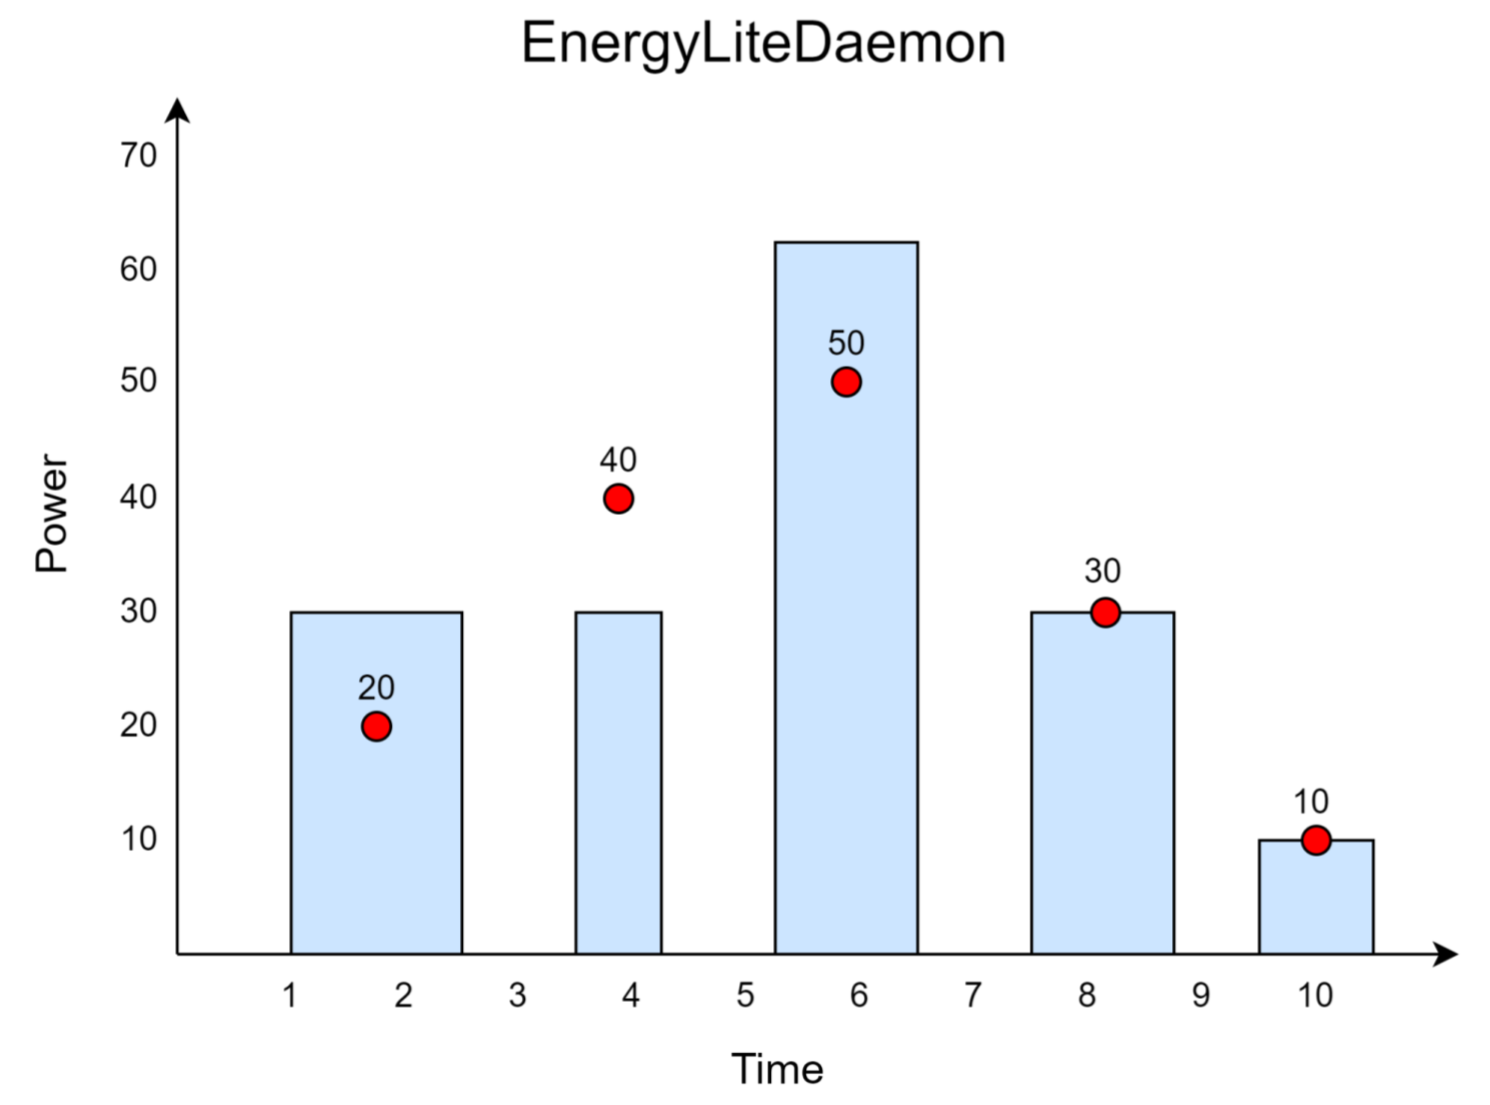
\includegraphics[width=\textwidth]{imgs/EnergyLiteDaemon_Energy_2.png}
         \caption{}
         \label{fig:c}
   \end{subfigure}
   \hfill
   \begin{subfigure}[b]{0.24\textwidth} % Adjusted width
         \centering
         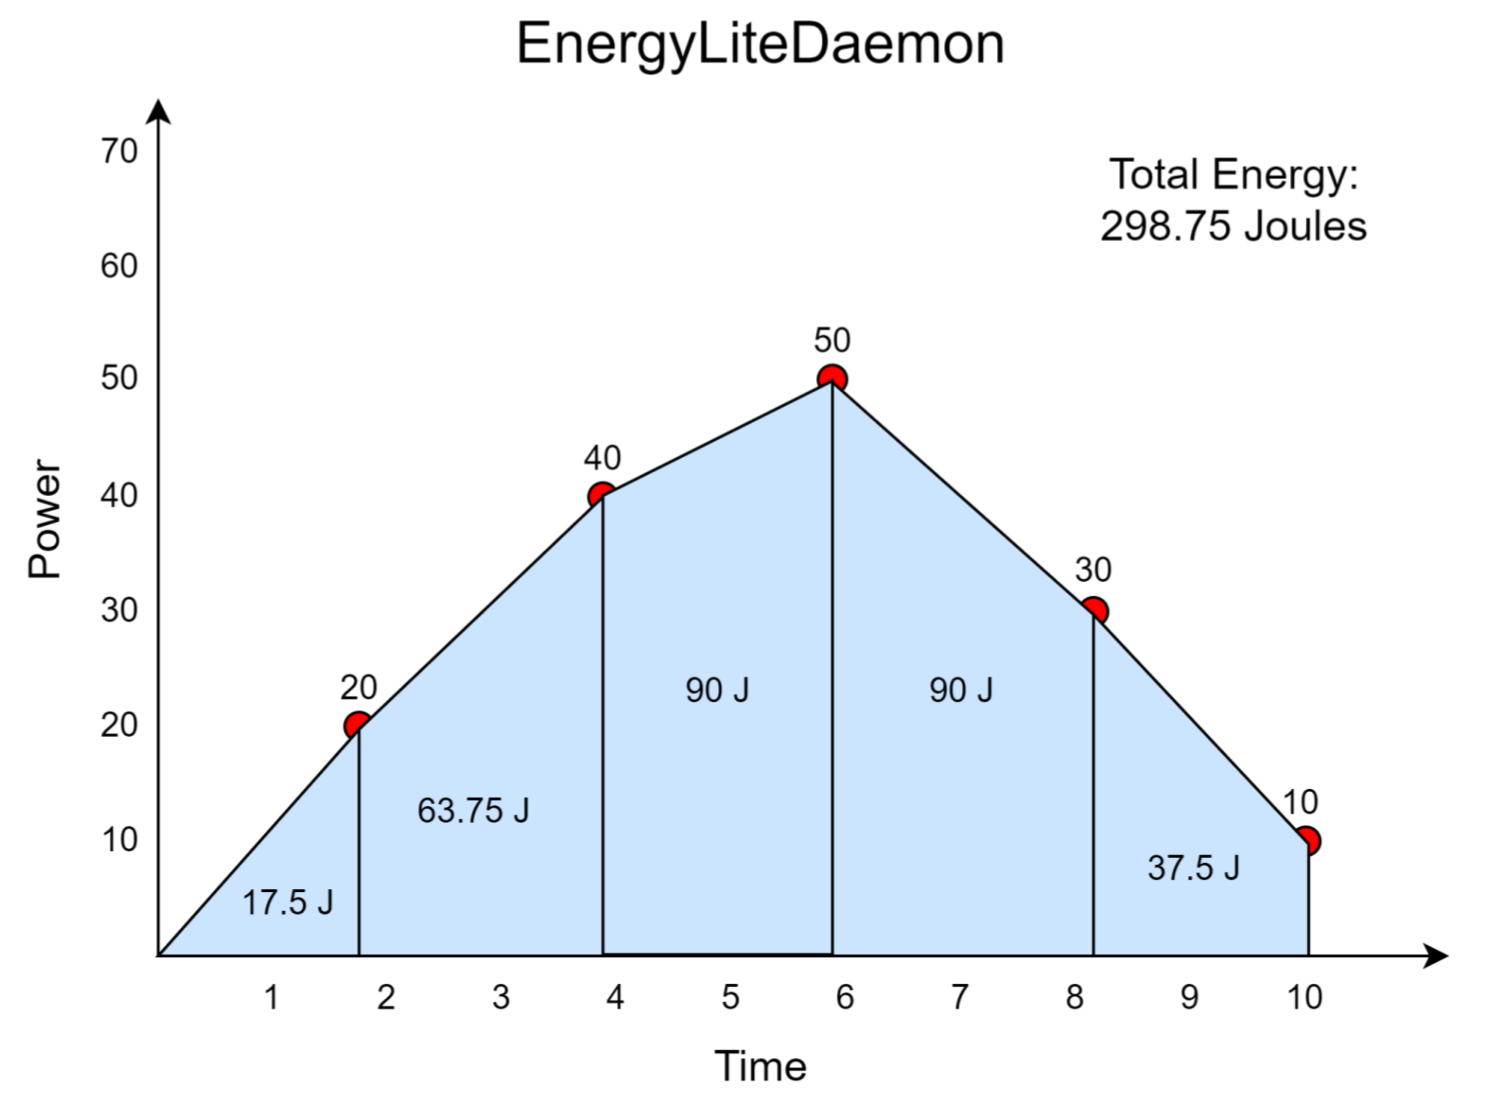
\includegraphics[width=\textwidth]{imgs/EnergyLiteDaemon_Energy_3.png}
         \caption{}
         \label{fig:d}
   \end{subfigure}
   
   \caption{Toy example of energy measurement of a container using EnergAt and EnergyLiteDaemon. (a) EnergAt energy readings. (b) EnergyLiteDaemon energy readings. (c) EnergyLiteDaemon power calculation (red dots). (d) EnergyLiteDaemon energy interpolation using trapezoidal integration.}
   \label{fig:energy_toy_example}
\end{figure*}



\subsection{Energy Variation with vCPU and Frequency Allocation}
\label{appendix:energy_variation_vcpu_frequency}
The energy usage and duration Float Matrix Multiplication, Image Processing, and Encryption as a function of vCPU allocation and frequency are shown in Figure \ref{fig:energy_duration_heatmaps}. 

The maximum CPU usage for Float Matrix Multiplication, Image Processing, and Encryption as a function of vCPU count are shown in Figure \ref{fig:max_cpu}. 

\begin{figure*}[ht]
   \centering
   % First row of plots
   % \textbf{Spin Up Stage}\par\medskip
   \begin{subfigure}[b]{0.33\textwidth}
     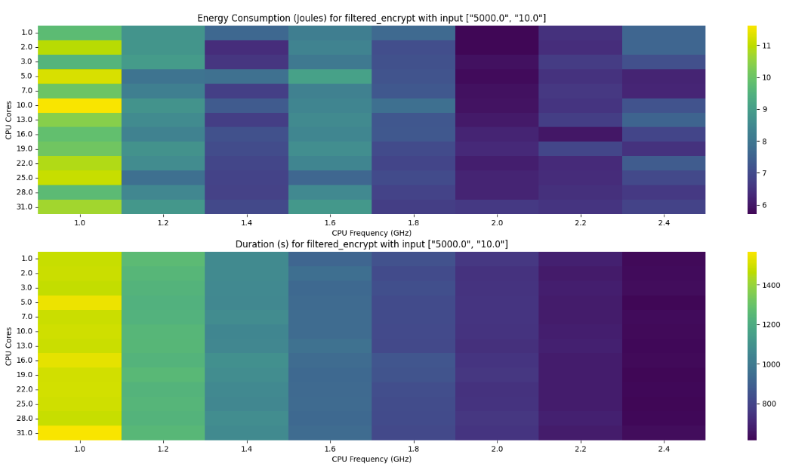
\includegraphics[width=\textwidth]{imgs/study_1_results/heatmaps/energy_encrypt.png}
     \caption{Encrypt}
     \label{fig:energy_encrypt}
   \end{subfigure}
   \hfill
   \begin{subfigure}[b]{0.33\textwidth}
      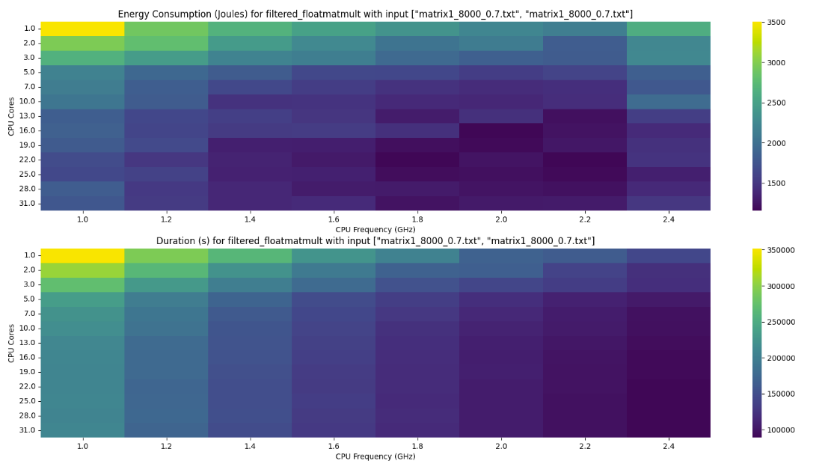
\includegraphics[width=\textwidth]{imgs/study_1_results/heatmaps/energy_floatmatmult.png}
     \caption{Float Matrix Multiplication}
     \label{fig:energy_floatmatmult}
   \end{subfigure}
   \hfill
   \begin{subfigure}[b]{0.33\textwidth}
      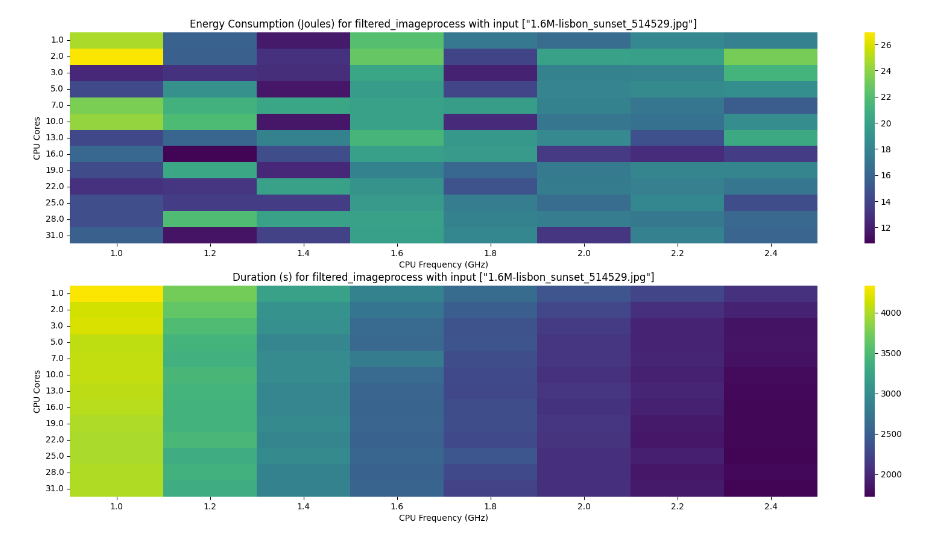
\includegraphics[width=\textwidth]{imgs/study_1_results/heatmaps/energy_image.png}
     \caption{Image Processing}
     \label{fig:energy_image}
   \end{subfigure}
   \caption{Heatmaps for energy (top plot) and duration (bottom plot) as a function of vCPU frequency (x-axis) and vCPU count (y-axis)}
   \label{fig:energy_duration_heatmaps} % Move this line inside the figure environment
\end{figure*}

\begin{figure*}[ht]
   \centering
   % First row of plots
   % \textbf{Spin Up Stage}\par\medskip
   \begin{subfigure}[b]{0.33\textwidth}
     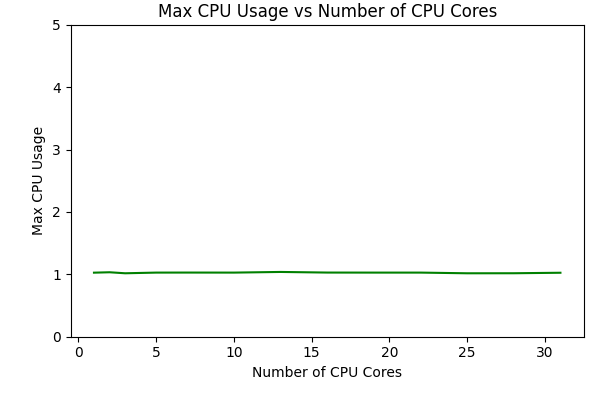
\includegraphics[width=\textwidth]{imgs/study_1_results/var_cpu/encryption/CPU_CPUUsage.png}
     \caption{Encrypt}
     \label{fig:encrypt_max_cpu}
   \end{subfigure}
   \hfill
   \begin{subfigure}[b]{0.33\textwidth}
      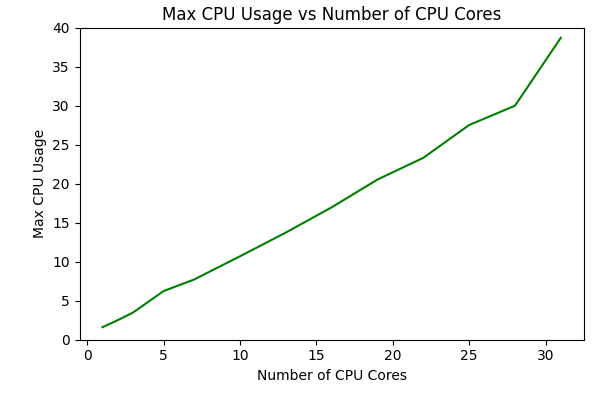
\includegraphics[width=\textwidth]{imgs/study_1_results/var_cpu/floatmatmul/CPU_CPUUsage.png}
     \caption{Float Matrix Multiplication}
     \label{fig:floatmatmult_max_cpu}
   \end{subfigure}
   \hfill
   \begin{subfigure}[b]{0.33\textwidth}
      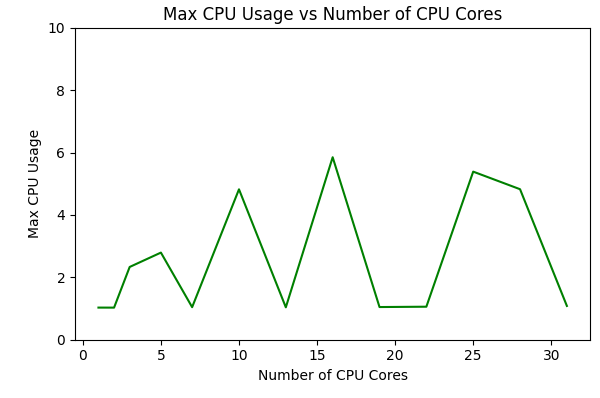
\includegraphics[width=\textwidth]{imgs/study_1_results/var_cpu/imageprocess/CPU_CPUUsage.png}
     \caption{Image Processing}
     \label{fig:image_max_cpu}
   \end{subfigure}
   \caption{Max CPU usage as a function of vCPU count}
   \label{fig:max_cpu} % Move this line inside the figure environment
\end{figure*}




 \subsection{Energy Variation for Different Stages of a Serverless Function Invocation}
 \label{appendix:energy_variation_vcpu_memory}
 We can see that the energy consumption of the container spin-up, idle time, and container spin-down for different image sizes in Figure \ref{fig:energy_stages}. 

 \begin{figure*}[ht]
   \centering
   % First row of plots
   \textbf{Spin Up Stage}\par\medskip
   \begin{subfigure}[b]{0.3\textwidth}
     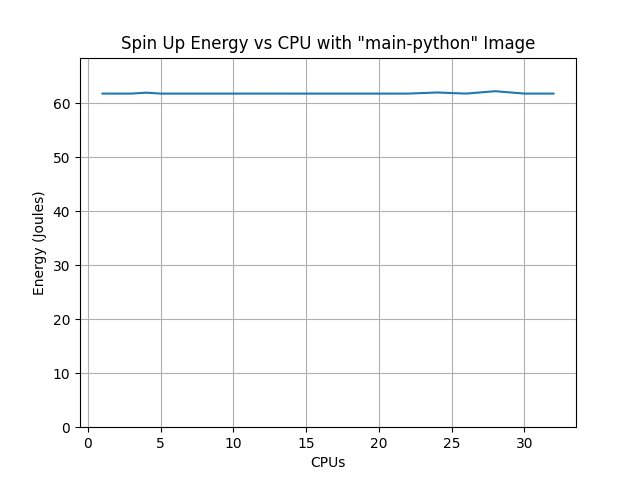
\includegraphics[width=\textwidth]{imgs/container_study/spin_up_vs_cpu.png}
     \caption{}
     \label{fig:spin_up_cpu}
   \end{subfigure}
   \hfill
   \begin{subfigure}[b]{0.3\textwidth}
      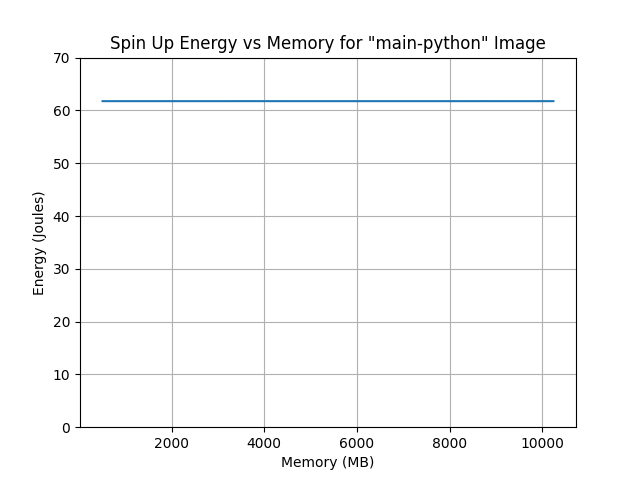
\includegraphics[width=\textwidth]{imgs/container_study/spin_up_vs_mem.png}
     \caption{}
     \label{fig:spin_up_mem}
   \end{subfigure}
   \hfill
   \begin{subfigure}[b]{0.3\textwidth}
      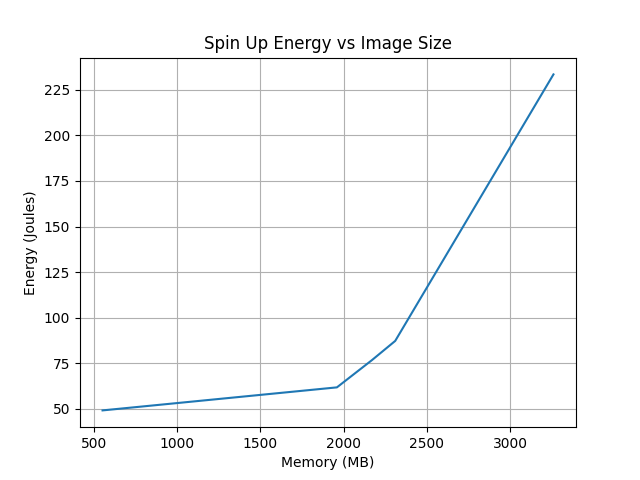
\includegraphics[width=\textwidth]{imgs/container_study/spin_up_vs_image.png}
     \caption{}
     \label{fig:spin_up_img}
   \end{subfigure}
   % \caption*{Float Matrix Multiplication}
   
   % Second row of plots
   \textbf{Spin Down Stage}\par\medskip
   \begin{subfigure}[b]{0.3\textwidth}
      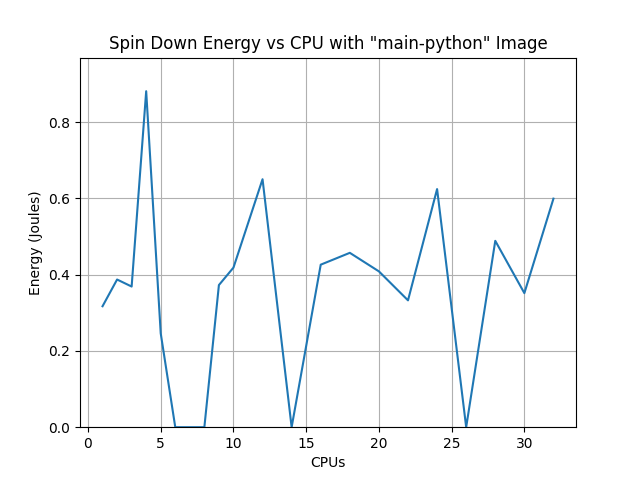
\includegraphics[width=\textwidth]{imgs/container_study/spin_down_vs_cpu.png}
     \caption{}
     \label{fig:spin_down_cpu}
   \end{subfigure}
   \hfill
   \begin{subfigure}[b]{0.3\textwidth}
      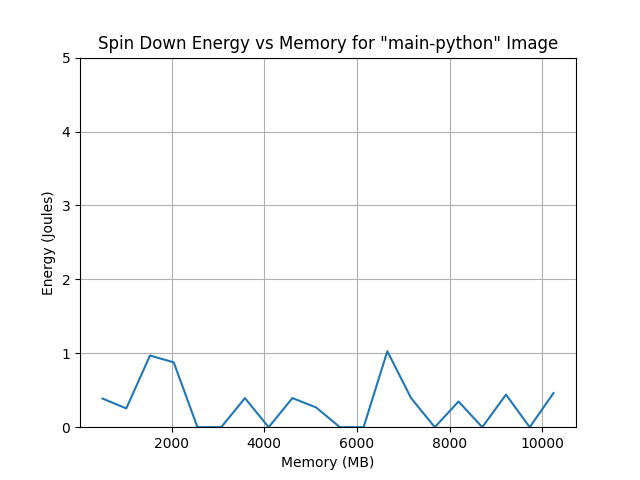
\includegraphics[width=\textwidth]{imgs/container_study/spin_down_vs_mem.png}
     \caption{}
     \label{fig:spin_down_mem}
   \end{subfigure}
   \hfill
   \begin{subfigure}[b]{0.3\textwidth}
      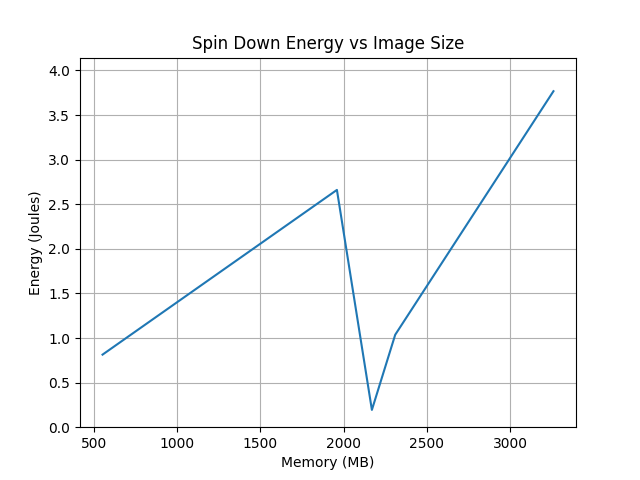
\includegraphics[width=\textwidth]{imgs/container_study/spin_down_vs_image.png}
     \caption{}
     \label{fig:spin_down_img}
   \end{subfigure}
   % \caption*{Image Process}
   
   % Third row of plots
   \textbf{Idle Stage}\par\medskip
   \begin{subfigure}[b]{0.3\textwidth}
      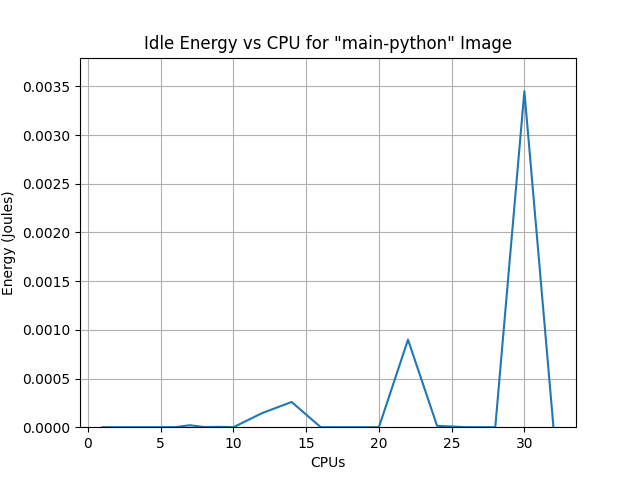
\includegraphics[width=\textwidth]{imgs/container_study/idle_vs_cpu.png}
     \caption{}
     \label{fig:idle_cpu}
   \end{subfigure}
   \hfill
   \begin{subfigure}[b]{0.3\textwidth}
      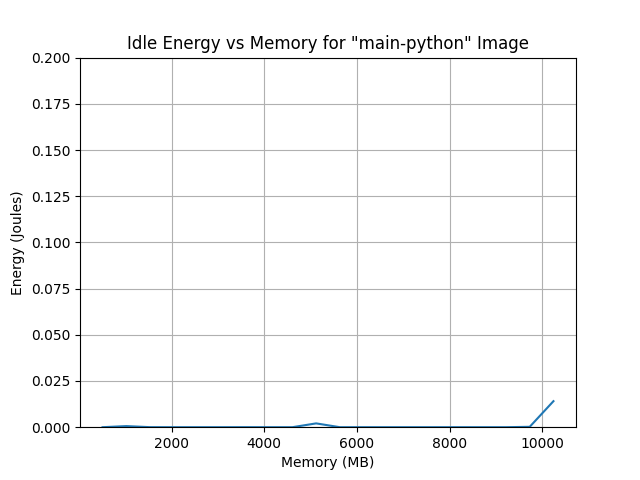
\includegraphics[width=\textwidth]{imgs/container_study/idle_vs_mem.png}
     \caption{}
     \label{fig:idle_mem}
   \end{subfigure}
   \hfill
   \begin{subfigure}[b]{0.3\textwidth}
      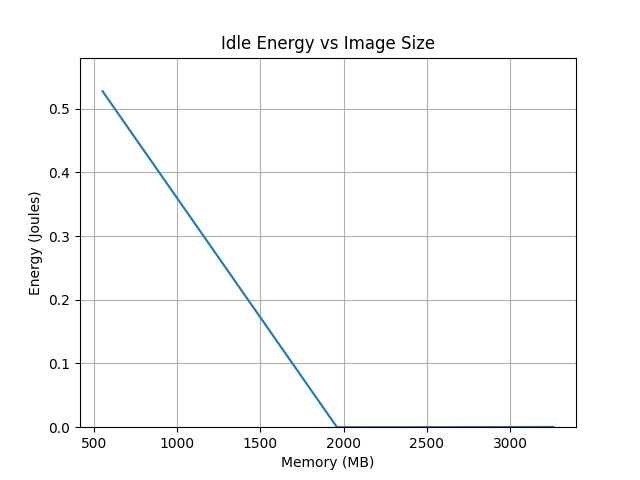
\includegraphics[width=\textwidth]{imgs/container_study/idle_vs_img.png}
     \caption{}
     \label{fig:idle_img}
   \end{subfigure}
   % \caption*{Encryption}
   
   \caption{Energy Usage vs CPU (a, d, g), Memory (b, e, h), and Image Size (c, f, i) for the Spin Up, Spin Down, and Idle stages of a serverless function invocation.}
   \label{fig:energy_stages}
 \end{figure*}


 
 \subsection{Evaluation of the Performance of Gaussian Process Regression Model on Measurement Study Data }
 \label{appendix:regression_model_measurement_study}

 For each function type and a few fixed input, we can see the energy per invocation over time, along with the difference between the predicted energy and the actual energy of the output configuration, and the difference between the actual energy of the output configuration and the ground truth minimum in Figure \ref{fig:model_performance_measurement_study_} and \ref{fig:model_performance_measurement_study}


\begin{figure*}[ht]
   \centering
   % First row of plots
   \textbf{Float Matrix Multiplication}\par\medskip
   \begin{subfigure}[b]{0.22\textwidth}
     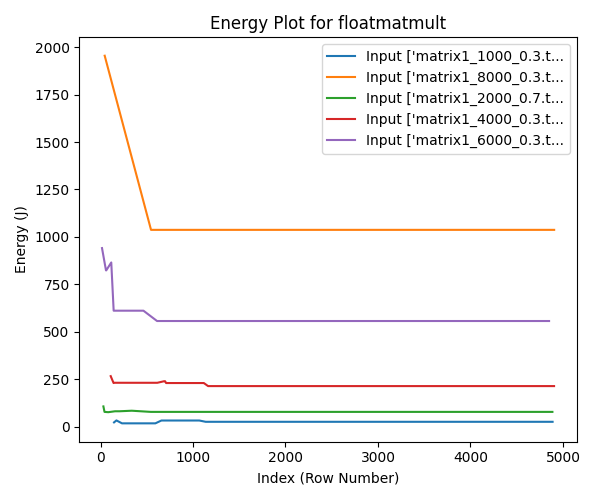
\includegraphics[width=\textwidth]{imgs/final_experiment_plots/model_analysis/measurement_data_analysis/matmult_energy.png}
     \caption{}
     \label{fig:matmultenergy}
   \end{subfigure}
   \hfill
   \begin{subfigure}[b]{0.22\textwidth}
      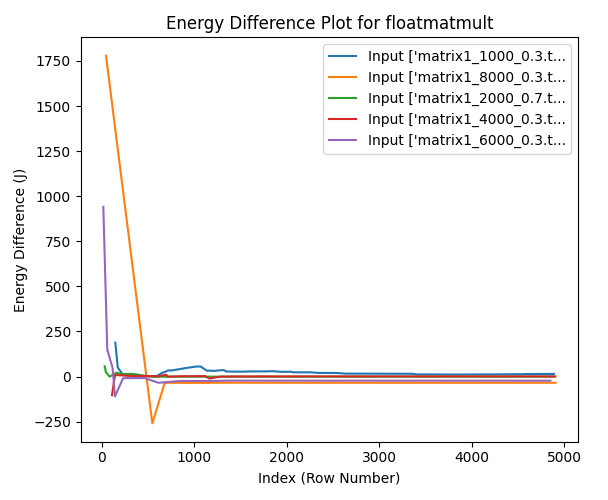
\includegraphics[width=\textwidth]{imgs/final_experiment_plots/model_analysis/measurement_data_analysis/matmult_energy_diff.png}
     \caption{}
     \label{fig:matmult_energy_diff}
   \end{subfigure}
   \hfill
   \begin{subfigure}[b]{0.22\textwidth}
      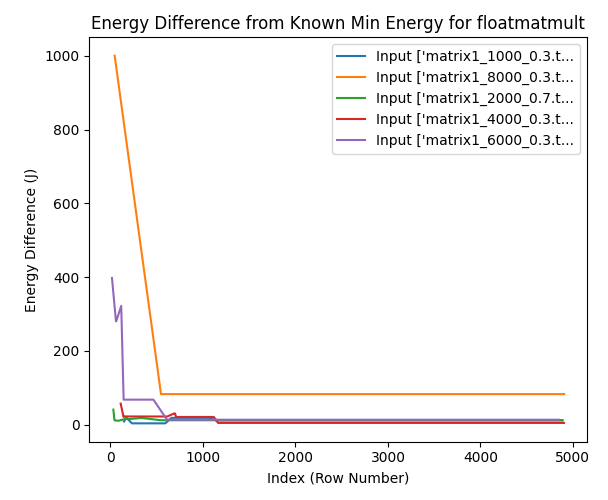
\includegraphics[width=\textwidth]{imgs/final_experiment_plots/model_analysis/measurement_data_analysis/matmult_compare_min.png}
     \caption{}
     \label{fig:matmult_comparemin}
   \end{subfigure}
   
   % Second row of plots
   \textbf{Linpack}\par\medskip
   \begin{subfigure}[b]{0.22\textwidth}
      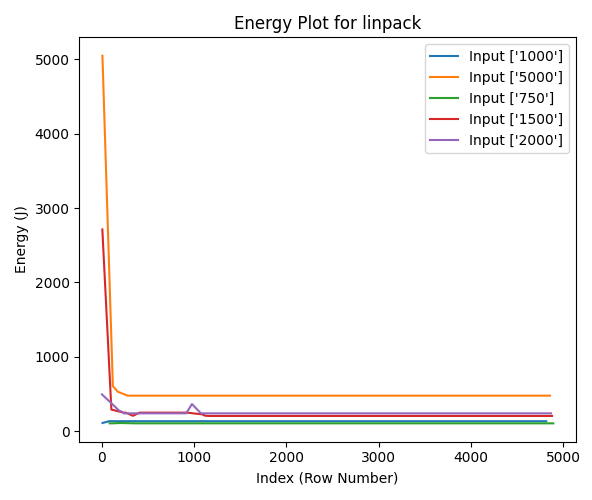
\includegraphics[width=\textwidth]{imgs/final_experiment_plots/model_analysis/measurement_data_analysis/linpack_energy.png}
     \caption{}
     \label{fig:linpack_energy}
   \end{subfigure}
   \hfill
   \begin{subfigure}[b]{0.22\textwidth}
      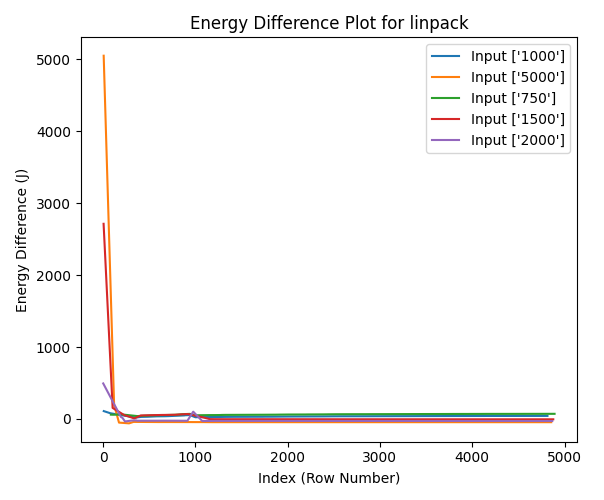
\includegraphics[width=\textwidth]{imgs/final_experiment_plots/model_analysis/measurement_data_analysis/linpack_energy_diff.png}
     \caption{}
     \label{fig:linpack_energy_diff}
   \end{subfigure}
   \hfill
   \begin{subfigure}[b]{0.22\textwidth}
      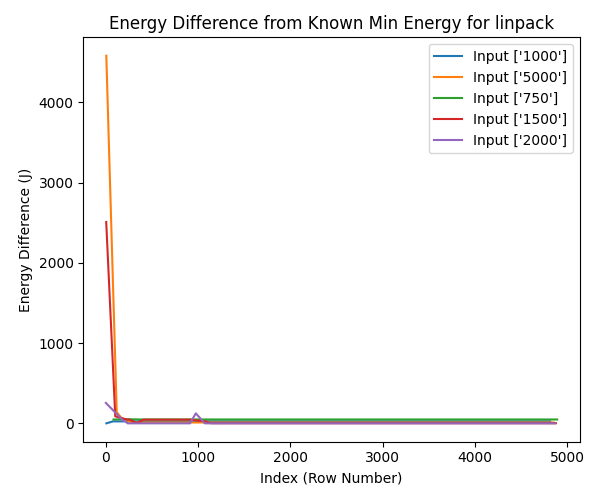
\includegraphics[width=\textwidth]{imgs/final_experiment_plots/model_analysis/measurement_data_analysis/linpack_compare_min.png}
     \caption{}
     \label{fig:linpack_compare_min}
   \end{subfigure}
   
   % Third row of plots
   \textbf{Encrypt}\par\medskip
   \begin{subfigure}[b]{0.22\textwidth}
      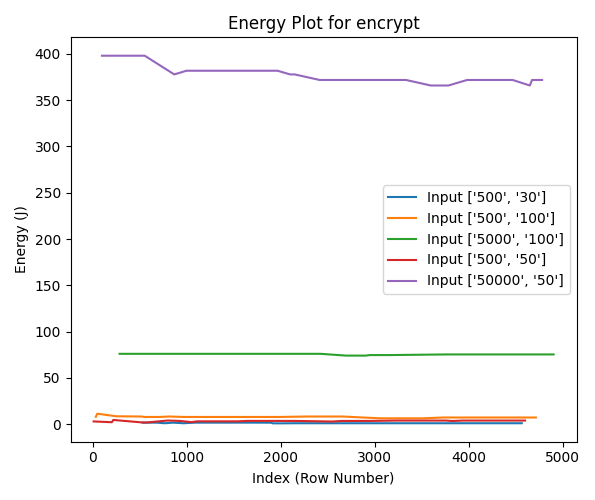
\includegraphics[width=\textwidth]{imgs/final_experiment_plots/model_analysis/measurement_data_analysis/encrypt_energy.png}
     \caption{}
     \label{fig:encrypt_energy}
   \end{subfigure}
   \hfill
   \begin{subfigure}[b]{0.22\textwidth}
      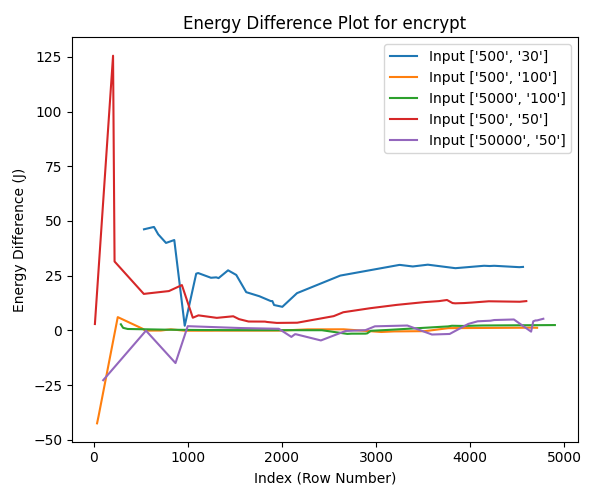
\includegraphics[width=\textwidth]{imgs/final_experiment_plots/model_analysis/measurement_data_analysis/encrypt_energy_diff.png}
     \caption{}
     \label{fig:encrypt_energy_diff}
   \end{subfigure}
   \hfill
   \begin{subfigure}[b]{0.22\textwidth}
      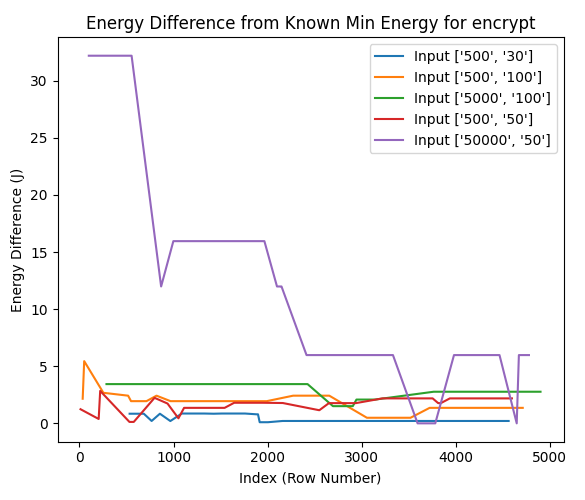
\includegraphics[width=\textwidth]{imgs/final_experiment_plots/model_analysis/measurement_data_analysis/encrypt_compare_min.png}
     \caption{}
     \label{fig:encrypt_compare_min}
   \end{subfigure}

   \caption{For each Floatmatmult, Encrypt, and Linpack: 1) Energy of a function invocation over time 2) Difference predicted energy and actual energy for predicted configuration for invocation over time 3) Difference between energy of predicted configuration and ground truth minimum energy for invocation over time}
   \label{fig:model_performance_measurement_study_}
\end{figure*}
\begin{figure*}[ht]
   \centering
   \newpage
   \newpage
   % Fourth row of plots
   \textbf{Image Processing}\par\medskip
   \begin{subfigure}[b]{0.22\textwidth}
      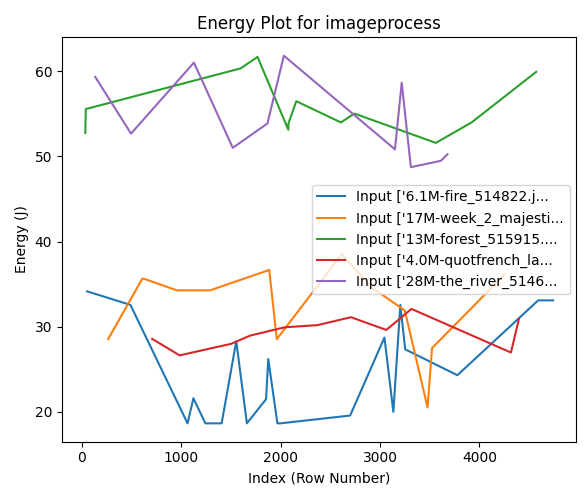
\includegraphics[width=\textwidth]{imgs/final_experiment_plots/model_analysis/measurement_data_analysis/image_energy.png}
     \caption{}
     \label{fig:image_energy}
   \end{subfigure}
   \hfill
   \begin{subfigure}[b]{0.22\textwidth}
      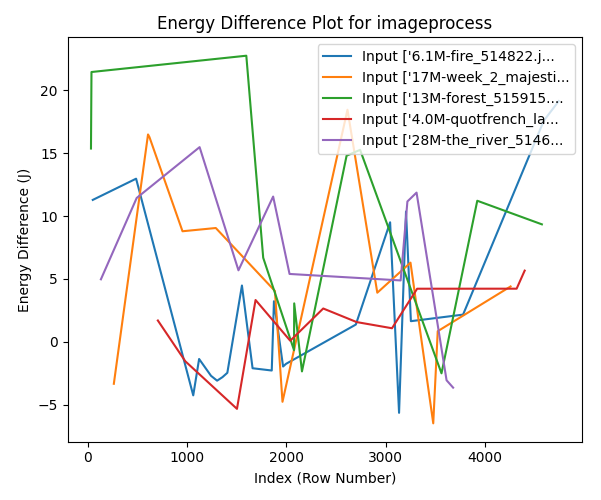
\includegraphics[width=\textwidth]{imgs/final_experiment_plots/model_analysis/measurement_data_analysis/image_energy_diff.png}
     \caption{}
     \label{fig:image_energy_diff}
   \end{subfigure}
   \hfill
   \begin{subfigure}[b]{0.22\textwidth}
      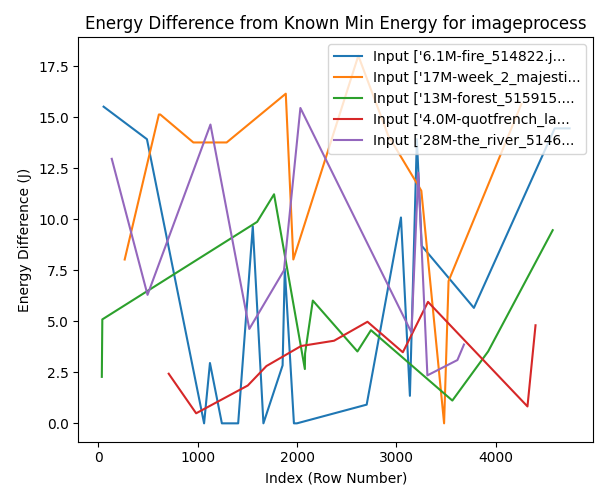
\includegraphics[width=\textwidth]{imgs/final_experiment_plots/model_analysis/measurement_data_analysis/image_compare_min.png}
     \caption{}
     \label{fig:image_compare_min}
   \end{subfigure}

   % Fifth row of plots
   \textbf{Video Processing}\par\medskip
   \begin{subfigure}[b]{0.22\textwidth}
      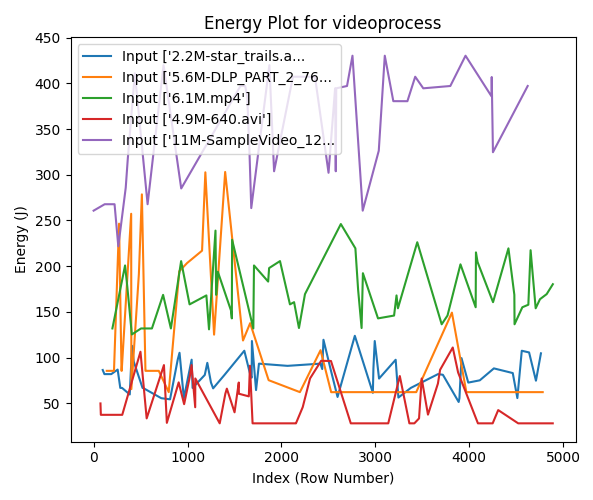
\includegraphics[width=\textwidth]{imgs/final_experiment_plots/model_analysis/measurement_data_analysis/video_energy.png}
     \caption{}
     \label{fig:video_energy}
   \end{subfigure}
   \hfill
   \begin{subfigure}[b]{0.22\textwidth}
      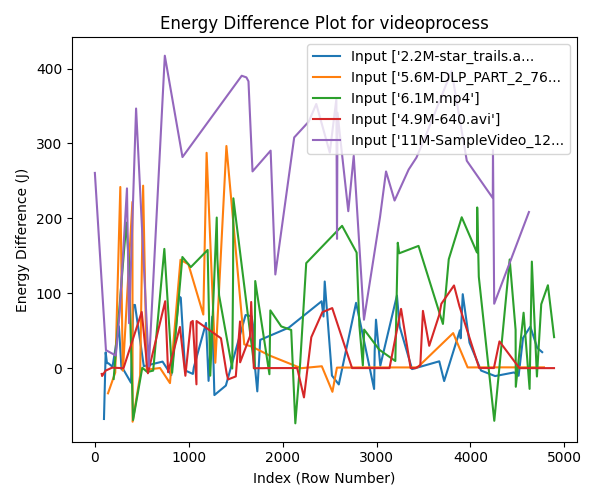
\includegraphics[width=\textwidth]{imgs/final_experiment_plots/model_analysis/measurement_data_analysis/video_energy_diff.png}
     \caption{}
     \label{fig:video_energy_diff}
   \end{subfigure}
   \hfill
   \begin{subfigure}[b]{0.22\textwidth}
      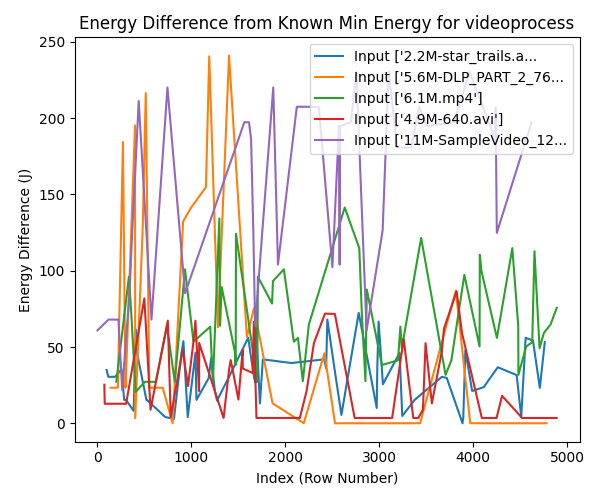
\includegraphics[width=\textwidth]{imgs/final_experiment_plots/model_analysis/measurement_data_analysis/video_compare_min.png}
     \caption{}
     \label{fig:video_compare_min}
   \end{subfigure}
   
   \caption{For each Image Processing and Video Processing: 1) Energy of a function invocation over time 2) Difference predicted energy and actual energy for predicted configuration for invocation over time 3) Difference between energy of predicted configuration and ground truth minimum energy for invocation over time}
   \label{fig:model_performance_measurement_study}
 \end{figure*}


  
 \subsection{Evaluation of the End-to-End System on an Azure Trace}
 \label{appendix:end-to-end_analysis}

 Figure \ref{fig:end_to_end_per_invocation_} and \ref{fig:end_to_end_per_invocation} shows the energy difference per invocation of a function type between CASS and the two baselines, Aquatope and Parrotfish. 

 \begin{figure*}[ht]
   \centering
   % First row of plots
   \textbf{Float Matrix Multiplication}\par\medskip
   \begin{subfigure}[b]{0.4\textwidth}
      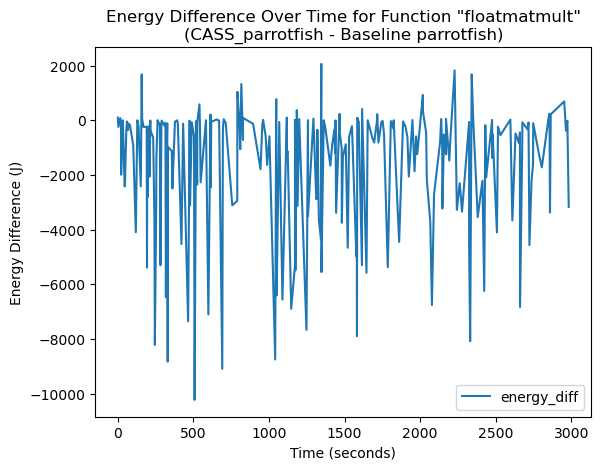
\includegraphics[width=\textwidth]{imgs/final_experiment_plots/energy_comparison/parrotfish/floatmatmult.png}
     \caption{}
     \label{fig:matmult_energy_diff_parrotfish}
   \end{subfigure}
   \hfill
   \begin{subfigure}[b]{0.4\textwidth}
      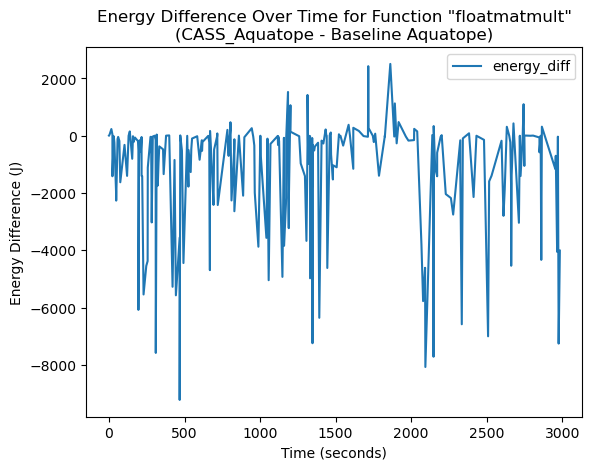
\includegraphics[width=\textwidth]{imgs/final_experiment_plots/energy_comparison/aquatope/floatmatmult.png}
     \caption{}
     \label{fig:matmult_energy_diff_aquatope}
   \end{subfigure}
   
   % Second row of plots
   \textbf{Linpack}\par\medskip
   \begin{subfigure}[b]{0.4\textwidth}
      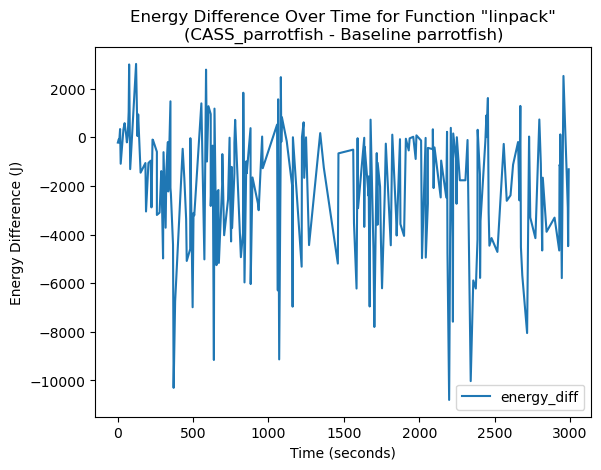
\includegraphics[width=\textwidth]{imgs/final_experiment_plots/energy_comparison/parrotfish/linpack.png}
     \caption{}
     \label{fig:linpack_energy_diff_parrotfish}
   \end{subfigure}
   \hfill
   \begin{subfigure}[b]{0.4\textwidth}
      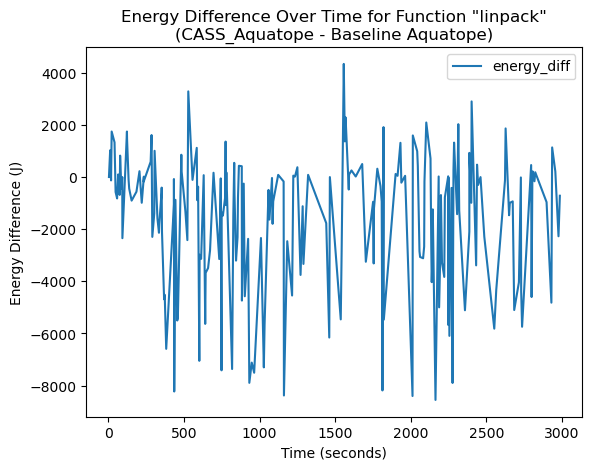
\includegraphics[width=\textwidth]{imgs/final_experiment_plots/energy_comparison/aquatope/linpack.png}
     \caption{}
     \label{fig:linpack_energy_diff_aquatope}
   \end{subfigure}
   
   % Third row of plots
   \textbf{Encrypt}\par\medskip
   \begin{subfigure}[b]{0.4\textwidth}
      \includegraphics[width=\textwidth]{imgs/final_experiment_plots/energy_comparison/parrotfish/encrypt.png}
     \caption{}
     \label{fig:encrypt_energy_diff_parrotfish}
   \end{subfigure}
   \hfill
   \begin{subfigure}[b]{0.4\textwidth}
      \includegraphics[width=\textwidth]{imgs/final_experiment_plots/energy_comparison/aquatope/encrypt.png}
     \caption{}
     \label{fig:encrypt_energy_diff_aquatope}
   \end{subfigure}
   
   \caption{For Floatmatmult, Encrypt, and Linpack, we show the energy difference per invocation between CASS and 1) Parrotfish and 2) Aquatope}
   \label{fig:end_to_end_per_invocation_}
 \end{figure*}

\begin{figure*}[ht]
   \centering
   \newpage
   \newpage
   % Fourth row of plots
   \textbf{Image Processing}\par\medskip
   \begin{subfigure}[b]{0.4\textwidth}
      \includegraphics[width=\textwidth]{imgs/final_experiment_plots/energy_comparison/parrotfish/imageprocess.png}
     \caption{}
     \label{fig:image_energy_diff_parrotfish}
   \end{subfigure}
   \hfill
   \begin{subfigure}[b]{0.4\textwidth}
      \includegraphics[width=\textwidth]{imgs/final_experiment_plots/energy_comparison/aquatope/imageprocess.png}
     \caption{}
     \label{fig:image_energy_diff_aquatope}
   \end{subfigure}

   \textbf{Video Processing}\par\medskip
   \begin{subfigure}{0.4\textwidth}
      \includegraphics[width=\textwidth]{imgs/final_experiment_plots/energy_comparison/parrotfish/videoprocess.png}
     \caption{}
     \label{fig:video_energy_diff_parrotfish}
   \end{subfigure}
   \hfill
   \begin{subfigure}{0.4\textwidth}
      \includegraphics[width=\textwidth]{imgs/final_experiment_plots/energy_comparison/aquatope/videoprocess.png}
     \caption{}
     \label{fig:video_energy_diff_aquatope}
   \end{subfigure}
   \caption{For Image Processing and Video Processing, we show the energy difference per invocation between CASS and 1) Parrotfish and 2) Aquatope}
   \label{fig:end_to_end_per_invocation}
   
\end{figure*}


\end{document}
